\documentclass[acmsmall,screen]{acmart}
% Packages and definitions for the acmart (ACM Computing Surveys) build.
% acmart already loads amsmath, xcolor, graphicx, hyperref, natbib and booktabs; layout and fonts are
% fixed by the class and are not changed here.
\usepackage{tabularx,multirow,array}
\usepackage{adjustbox}
\usepackage{subcaption}
\usepackage{enumitem}
\usepackage[most]{tcolorbox}
\usepackage{tikz}
\usetikzlibrary{arrows.meta,positioning,fit,backgrounds,calc,shapes.geometric,shapes.misc,decorations.pathreplacing}
\usepackage[nameinlink,capitalise,noabbrev]{cleveref}

% Palette shared by all figures (six functional categories; validated for colour-vision deficiency,
% always paired with text labels).
\definecolor{encode}{HTML}{2A78D6}
\definecolor{anticipate}{HTML}{EB6834}
\definecolor{compute}{HTML}{1BAF7A}
\definecolor{provision}{HTML}{6250D6}
\definecolor{connect}{HTML}{E87BA4}
\definecolor{assure}{HTML}{008300}
\definecolor{gapcolor}{HTML}{B03A2E}

\setlist{itemsep=1pt,topsep=3pt}
\graphicspath{{figures/}}

\newtcolorbox{openproblemsbox}{breakable,enhanced,colback=gapcolor!3,colframe=gapcolor!65!black,
  boxrule=0.6pt,arc=1.5pt,fonttitle=\bfseries\sffamily\small,title={Open problems},
  left=5pt,right=5pt,top=3pt,bottom=3pt}
\newenvironment{openproblems}{\begin{openproblemsbox}\small\begin{enumerate}[label=\textbf{P\arabic*.},leftmargin=2em,itemsep=2pt]}{\end{enumerate}\end{openproblemsbox}}
\setlength{\emergencystretch}{1.5em}


\setcopyright{none}
\acmJournal{CSUR}
\acmYear{2026}

\begin{document}

\title{Carrying Immersion over Networks: A Survey of Networked Extended Reality}

\author{Anonymous}
\affiliation{%
  \institution{To be completed}
  \city{}
  \country{To be completed}}

\begin{abstract}
Extended reality (XR) puts the network inside a perceptual loop. When the user's head turns, the new view
must appear within a few tens of milliseconds. Once content, computation or other participants are
remote, the network must carry 360-degree and volumetric media at high rates, return rendered frames
inside that deadline, take a continuous uplink of pose and sensor data, and keep several people and
machines consistent. This survey organises networked XR by the six functions that every such system
performs. It must \emph{encode} the scene into something that can be sent, \emph{anticipate} what the
user will need next, decide where to \emph{compute}, \emph{provision} the network, \emph{connect} people
and machines that share a world, and \emph{assure} that the experience is good enough and safe. For each
function we state the design question and group the approaches into families by their underlying idea.
We then separate what has been established on real systems from what is contested and what is merely
assumed. Two couplings tie the functions together: a shared deadline that every function spends from,
and a trade between network and device that every design shifts one way or the other. Across all six
functions the same weaknesses recur. Objectives are rarely validated against what users perceive,
requirement figures are inherited rather than measured, and controllers are seldom tested beyond the
simulator. The uplink, multi-user scale and the latency cost of security are studied least. We close
with nine cross-cutting gaps and a dependency-ordered research agenda.
\end{abstract}


\begin{CCSXML}
<ccs2012>
<concept><concept_id>10003033.10003079</concept_id><concept_desc>Networks~Network performance evaluation</concept_desc><concept_significance>300</concept_significance></concept>
<concept><concept_id>10003033.10003106.10003113</concept_id><concept_desc>Networks~Mobile networks</concept_desc><concept_significance>500</concept_significance></concept>
<concept><concept_id>10003120.10003121.10003124.10010866</concept_id><concept_desc>Human-centered computing~Virtual reality</concept_desc><concept_significance>500</concept_significance></concept>
<concept><concept_id>10003120.10003121.10003124.10010392</concept_id><concept_desc>Human-centered computing~Mixed / augmented reality</concept_desc><concept_significance>300</concept_significance></concept>
<concept><concept_id>10002951.10003227.10003251</concept_id><concept_desc>Information systems~Multimedia information systems</concept_desc><concept_significance>300</concept_significance></concept>
</ccs2012>
\end{CCSXML}
\ccsdesc[500]{Networks~Mobile networks}
\ccsdesc[300]{Networks~Network performance evaluation}
\ccsdesc[500]{Human-centered computing~Virtual reality}
\ccsdesc[300]{Human-centered computing~Mixed / augmented reality}
\ccsdesc[300]{Information systems~Multimedia information systems}

\keywords{extended reality, virtual reality, augmented reality, 360-degree video, volumetric video,
viewport prediction, edge computing, remote rendering, split rendering, motion-to-photon latency, 5G, 6G,
tactile internet, holographic communication, quality of experience}

\maketitle

\section{Introduction}\label{sec:intro}

A head-mounted display shows a world that must respond to the head that wears it. When the user turns,
the new view must appear within a few tens of milliseconds, or the image lags the body and comfort
fails \cite{W2784711283}. On a standalone device this deadline is met locally. Once the scene, the
computation or the other participants are elsewhere, the network becomes part of the perceptual loop.
Extended reality (XR), the umbrella term for virtual, augmented and mixed reality, therefore asks more of
a network than video or the web. A 360-degree or volumetric stream needs hundreds of megabits per second
if it is sent whole \cite{W3038754372,W3096564590}. Remote rendering must finish a frame within the
motion-to-photon (MTP) budget \cite{W2784711283}. The device sends pose, camera frames and captured media
upstream all the time. When several people share a world, the network must also keep them consistent
with each other \cite{W2561715836}.

Ten years of research have produced many answers to these demands, and they are scattered across
communities that seldom read each other. Multimedia-systems researchers built viewport-adaptive
streaming. Mobile-computing researchers offloaded AR recognition to the edge \cite{W3133913697}. Wireless
researchers framed XR as a joint allocation of radio, computing and energy. Haptics researchers pursued
the tactile internet \cite{W2811040154}. Visionaries placed all of it inside 6G and the metaverse
\cite{W4312940001,W4390204075}. Existing surveys follow these boundaries. Each covers one medium, such as
360-degree video \cite{W3038754372,W2971680322,W2917103012}, point clouds \cite{W3096564590} or haptics
\cite{W3088582486}, or one technology, such as edge computing \cite{W3133913697,W2902319104}, ultra-low
latency \cite{W4362585626} or the 6G metaverse \cite{W4312940001,W4315497913}. None measures the field as
a whole, and none asks how well its claims are tested.

This review does both. It condenses the \emph{Networked XR Atlas}, a corpus of \nxrIncluded{} papers
published between October 2016 and October 2026. The atlas was screened from \nxrHarvested{} records
with a validated procedure, labelled on five dimensions and read in depth where it mattered most
(Section~\ref{sec:method}). The atlas supports three kinds of statement: counts and trends over the whole
corpus, syntheses of the papers that shape each topic, and gaps that have been checked against a text
search of every included paper.

\paragraph{Organising idea.} We do not organise the field by technology or by medium. We organise it by
\emph{function}: the six things any networked XR system must do, whatever its medium and access network
(Section~\ref{sec:framework}). A system must \emph{encode} the scene into something that can be sent
(Section~\ref{sec:encode}). It must \emph{anticipate} what the user will look at or do next, so that the
right content arrives in time (Section~\ref{sec:anticipate}). It must decide where to \emph{compute}, on
the device, at the edge or in the cloud, and how to hide the delay this adds (Section~\ref{sec:compute}).
It must \emph{provision} the network with radio, scheduling, transport and architecture that supply the
rate, delay and reliability required (Section~\ref{sec:provision}). It must \emph{connect} users with each
other and with remote machines, through shared state, touch and telepresence (Section~\ref{sec:connect}).
And it must \emph{assure} that the result is good enough and safe for the people who use it
(Section~\ref{sec:assure}). Each function poses its own design question, and the answers can be compared
on the same terms.

\paragraph{Contributions.} The review makes four contributions.
\begin{enumerate}[leftmargin=*,label=(\arabic*)]
  \item A \textbf{functional taxonomy} of networked XR that places the \nxrNCatProb{} networking problems
        and \nxrNCatCont{} content types of the atlas codebook into six functions, each defined by a design
        question (Section~\ref{sec:framework}, \cref{fig:architecture,tab:framework}).
  \item A \textbf{quantitative account of how the field has changed}: its growth, the move from
        delivering content to allocating resources, the replacement of 360-degree video by generic XR
        traffic as the reference workload, and the decline of evaluation on real systems
        (Section~\ref{sec:landscape}).
  \item A \textbf{synthesis of each function} that separates what is established, what is contested and
        what is assumed, with the measured results that support each claim
        (Sections~\ref{sec:encode}--\ref{sec:assure}).
  \item \textbf{Nine cross-cutting gaps} and a research agenda ordered by dependency: which projects
        produce the data and models that the others need (Sections~\ref{sec:synthesis}
        and~\ref{sec:agenda}).
\end{enumerate}

\IfFileExists{sections/02_background.tex}{\section{Background: The Networked XR Loop}\label{sec:background}

This section introduces the concepts that the rest of the survey relies on. Readers familiar with XR
systems may skip to \cref{sec:framework}.

\subsection{From standalone to networked XR}
XR spans a continuum. Virtual reality (VR) replaces the user's view with a synthetic one. Augmented
reality (AR) overlays virtual objects on the physical world, and mixed reality anchors them in it so
that they respond to physical surfaces. Each device tracks the user's head, and often the hands and eyes,
and redraws the scene for every new pose. Two levels of freedom matter for networking. With \emph{three
degrees of freedom} (3DoF) the user can only rotate the head, as in a 360-degree video. With \emph{six
degrees of freedom} (6DoF) the user can also move through the scene, as in a game or a volumetric
capture. A 3DoF scene can be prepared in advance as a sphere of pixels. A 6DoF scene must be rendered or
synthesised for each viewpoint, so it needs either geometry on the device or rendering close to it.

A standalone headset performs the whole loop locally: it senses a pose, renders, and displays the result.
Three pressures push parts of this loop into the network. First, \emph{content} may be too large to
store, or may be produced live elsewhere, as with 360-degree broadcasts and volumetric captures. Second,
\emph{computation} may exceed what a light, battery-powered device can sustain, as with photorealistic
rendering and AR scene understanding \cite{W3133913697}. Third, \emph{other participants}, whether
people or machines, are by definition remote \cite{W2561715836}.

\subsection{The motion-to-photon deadline}
The defining constraint of XR is the \emph{motion-to-photon} (MTP) latency: the time from a head movement
to the photons that show its consequence. When MTP exceeds roughly 15--20~ms the displayed world appears
to lag or swim, which degrades presence and can cause simulator sickness. That budget leaves roughly
14~ms for computation and communication together \cite{W2784711283}. Three properties of this deadline
shape every design in this survey. First, it is \emph{per frame}: at 72--120 frames per second, each
frame has its own deadline, and a late frame is a lost frame. Second, it applies to \emph{rotation} most
strictly. Local reprojection can correct a slightly stale frame for a new head orientation, so the
network-facing deadline for full interaction is looser than MTP, although it is still tight. Third, its
\emph{tail} matters more than its mean, because occasional late frames are what users notice.

\subsection{What XR traffic looks like}
The traffic of a networked XR session differs from video streaming or web traffic in four ways
(\cref{tab:background}). It is \emph{periodic and bursty}: rendered or decoded frames arrive at the
display rate, each a burst of packets with its own deadline. It is \emph{bidirectional}: pose, controller
input, camera frames and captured media flow upstream continuously, and the downstream content depends on
them. It is \emph{viewport-dependent}: the user sees only a fraction of a 360-degree or volumetric scene
at any moment, so the useful content depends on where the user looks. And it is often \emph{shared}:
several users' updates must be reconciled into one consistent world. The first two properties make XR a
real-time control problem rather than a throughput problem. The third creates the opportunity to send
less. The fourth makes the network responsible for consistency as well as delivery.

\begin{table}[t]
\centering\small
\caption{How networked XR traffic differs from conventional video streaming. Each row names a
property, its consequence for the network, and the section that treats it.}\label{tab:background}
\setlength{\tabcolsep}{4pt}
\begin{tabularx}{\linewidth}{@{}>{\raggedright\arraybackslash}p{2.3cm}>{\raggedright\arraybackslash}X>{\raggedright\arraybackslash}X>{\raggedright\arraybackslash}p{1.9cm}@{}}
\toprule
Property & Video streaming & Networked XR & Treated in\\
\midrule
Deadline & Seconds of buffer absorb delay & Each frame must arrive within a few tens of milliseconds & \cref{sec:compute,sec:provision}\\
Direction & Downlink, with small requests upstream & Continuous uplink of pose, input, camera and capture & \cref{sec:compute,sec:connect}\\
Viewport & The whole frame is shown & Only the viewport is seen, and it moves & \cref{sec:anticipate}\\
Representation & 2D video frames & Spherical video, point clouds, meshes, neural fields, haptic signals & \cref{sec:encode}\\
Participants & Independent viewers & Shared state, avatars, remote machines & \cref{sec:connect}\\
Quality & Rebuffering, bitrate, video quality & Latency, judder, sickness, presence, task success & \cref{sec:assure}\\
\bottomrule
\end{tabularx}
\end{table}

\subsection{Where the loop can run}
A networked XR system distributes its loop over four tiers: the \emph{device}, the \emph{access network}
(Wi-Fi or cellular), the \emph{edge} (servers at or near the access network) and the \emph{cloud}. Moving
a function to a farther tier gains resources and loses time. An edge server one wireless hop away adds a
few milliseconds of round-trip time, while a distant cloud data centre adds tens of milliseconds
\cite{W2805833065}. Mobile edge computing, as standardised for 5G, exists largely to put rendering,
caching and session state within the XR deadline \cite{W2902319104}. The access network is usually the
least predictable part of the path. Wireless capacity, delay and loss vary with distance, blockage,
interference and the number of users, and a directional millimetre-wave beam must follow a head that
turns quickly. The framework in the next section builds on these four tiers.
}{}
\section{A Functional Framework for Networked XR}\label{sec:framework}

The atlas labels every paper by the networking problem it addresses and by the content it carries. These
labels are precise, but \nxrNCatProb{} problems and \nxrNCatCont{} content types are too many to reason
about together, and they mix levels: ``latency'' is a property, ``caching'' a mechanism and
``holographic communication'' an application. We therefore group them by \emph{function}, the job a
part of the system performs in the loop between the user's body and the content they perceive. A function
is defined by a design question that any networked XR system must answer, whatever its medium or access
network. \Cref{fig:architecture} places the six functions on a reference architecture, and
\cref{tab:framework} lists the atlas categories that each function contains.

\begin{figure}[t]
\centering
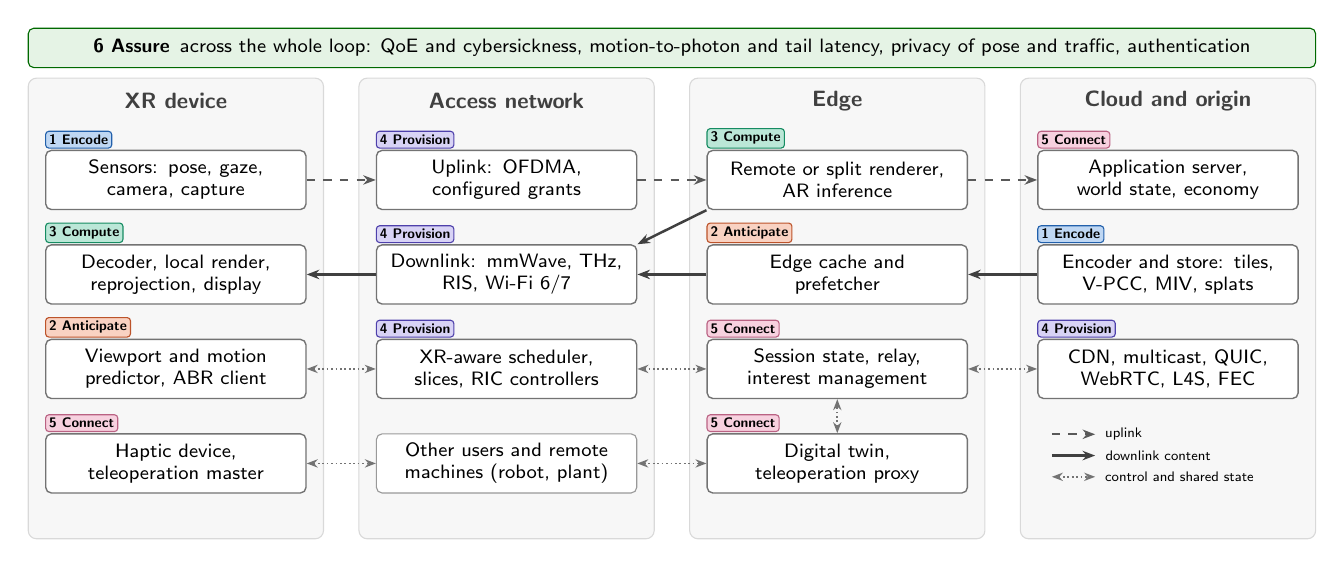
\begin{tikzpicture}[font=\sffamily\scriptsize,
  tier/.style={draw=black!15,fill=black!3,rounded corners=3pt,minimum width=3.75cm,minimum height=5.85cm,anchor=north},
  tierhead/.style={font=\sffamily\footnotesize\bfseries,text=black!75},
  comp/.style={draw=black!55,fill=white,rounded corners=2pt,align=center,minimum height=7.5mm,text width=3.2cm,inner sep=1.5pt,line width=0.5pt},
  fn/.style={rounded corners=1.2pt,font=\sffamily\tiny\bfseries,inner sep=1.3pt,text=black,anchor=south west,yshift=0.4pt},
  up/.style={-{Stealth[length=1.6mm]},line width=0.6pt,black!65,dashed},
  down/.style={-{Stealth[length=1.6mm]},line width=0.9pt,black!75},
  ctl/.style={{Stealth[length=1.4mm]}-{Stealth[length=1.4mm]},line width=0.6pt,black!55,densely dotted}]
  \def\X{{1.875,6.075,10.275,14.475}}
  \foreach \x/\name in {1.875/XR device,6.075/Access network,10.275/Edge,14.475/Cloud and origin}{
    \node[tier] at (\x,0) {};
    \node[tierhead] at (\x,-0.3) {\name};}
  % Row 1: uplink and interaction
  \node[comp] (sens) at (1.875,-1.3) {Sensors: pose, gaze,\\camera, capture};
  \node[comp] (ul)   at (6.075,-1.3) {Uplink: OFDMA,\\configured grants};
  \node[comp] (rend) at (10.275,-1.3) {Remote or split renderer,\\AR inference};
  \node[comp] (app)  at (14.475,-1.3) {Application server,\\world state, economy};
  % Row 2: downlink content
  \node[comp] (dec)  at (1.875,-2.5) {Decoder, local render,\\reprojection, display};
  \node[comp] (dl)   at (6.075,-2.5) {Downlink: mmWave, THz,\\RIS, Wi-Fi 6/7};
  \node[comp] (cache) at (10.275,-2.5) {Edge cache and\\prefetcher};
  \node[comp] (enc)  at (14.475,-2.5) {Encoder and store: tiles,\\V-PCC, MIV, splats};
  % Row 3: control and transport
  \node[comp] (pred) at (1.875,-3.7) {Viewport and motion\\predictor, ABR client};
  \node[comp] (sch)  at (6.075,-3.7) {XR-aware scheduler,\\slices, RIC controllers};
  \node[comp] (state) at (10.275,-3.7) {Session state, relay,\\interest management};
  \node[comp] (cdn)  at (14.475,-3.7) {CDN, multicast, QUIC,\\WebRTC, L4S, FEC};
  % Row 4: physical coupling
  \node[comp] (hap)  at (1.875,-4.9) {Haptic device,\\teleoperation master};
  \node[comp] (twin) at (10.275,-4.9) {Digital twin,\\teleoperation proxy};
  \node[draw=black!40,fill=white,rounded corners=2pt,align=center,text width=3.2cm,minimum height=7.5mm,inner sep=1.5pt] (peers) at (6.075,-4.9)
     {Other users and remote\\machines (robot, plant)};
  % Flows
  \draw[up] (sens) -- (ul); \draw[up] (ul) -- (rend); \draw[up] (rend) -- (app);
  \draw[down] (enc) -- (cache); \draw[down] (cache) -- (dl); \draw[down] (dl) -- (dec);
  \draw[down] (rend.south west) -- (dl.north east);
  \draw[ctl] (pred) -- (sch); \draw[ctl] (sch) -- (state); \draw[ctl] (state) -- (cdn);
  \draw[ctl] (hap) -- (peers); \draw[ctl] (peers) -- (twin); \draw[ctl] (twin) -- (state);
  % Function tags
  \node[fn,fill=encode!30,draw=encode!80!black] at (enc.north west) {1 Encode};
  \node[fn,fill=encode!30,draw=encode!80!black] at (sens.north west) {1 Encode};
  \node[fn,fill=anticipate!30,draw=anticipate!80!black] at (pred.north west) {2 Anticipate};
  \node[fn,fill=anticipate!30,draw=anticipate!80!black] at (cache.north west) {2 Anticipate};
  \node[fn,fill=compute!30,draw=compute!80!black] at (rend.north west) {3 Compute};
  \node[fn,fill=compute!30,draw=compute!80!black] at (dec.north west) {3 Compute};
  \node[fn,fill=provision!25,draw=provision!80!black] at (ul.north west) {4 Provision};
  \node[fn,fill=provision!25,draw=provision!80!black] at (dl.north west) {4 Provision};
  \node[fn,fill=provision!25,draw=provision!80!black] at (sch.north west) {4 Provision};
  \node[fn,fill=provision!25,draw=provision!80!black] at (cdn.north west) {4 Provision};
  \node[fn,fill=connect!35,draw=connect!80!black] at (state.north west) {5 Connect};
  \node[fn,fill=connect!35,draw=connect!80!black] at (twin.north west) {5 Connect};
  \node[fn,fill=connect!35,draw=connect!80!black] at (hap.north west) {5 Connect};
  \node[fn,fill=connect!35,draw=connect!80!black] at (app.north west) {5 Connect};
  % Assure band
  \node[draw=assure!80!black,fill=assure!10,rounded corners=2pt,minimum width=16.35cm,minimum height=5mm,anchor=south,
        font=\sffamily\scriptsize] at (8.175,0.12)
     {\textbf{6 Assure}\enspace across the whole loop: QoE and cybersickness, motion-to-photon and tail latency, privacy of pose and traffic, authentication};
  % Legend
  \begin{scope}[shift={(13.0,-4.75)},font=\sffamily\tiny]
    \draw[up] (0,0.22) -- (0.55,0.22) node[right,text=black]{uplink};
    \draw[down] (0,-0.05) -- (0.55,-0.05) node[right,text=black]{downlink content};
    \draw[ctl] (0,-0.32) -- (0.55,-0.32) node[right,text=black]{control and shared state};
  \end{scope}
\end{tikzpicture}
\caption{Reference architecture of a networked XR system, with the six functions placed where they act.
Rows read left to right as the uplink of pose and captured media, right to left as the downlink of
content, and as control and shared state that couple users and remote machines. The same function often
acts at several tiers: anticipation runs both on the device (prediction) and at the edge (caching), and
computation is split between device and edge.}\label{fig:architecture}
\end{figure}

\paragraph{The six functions.}
\begin{description}[leftmargin=0pt,itemsep=2pt,font=\normalfont\bfseries]
  \item[Encode] (\cref{sec:encode}). \emph{What representation of the scene travels, and how is it
        compressed?} Projections and tiling of 360-degree video, point clouds and meshes, multi-view
        video, neural scene representations, holograms and haptic signals.
  \item[Anticipate] (\cref{sec:anticipate}). \emph{What will the user need next, and how is it delivered
        in time?} Viewport-adaptive streaming, head, gaze and 6DoF motion prediction, and caching and
        prefetching.
  \item[Compute] (\cref{sec:compute}). \emph{Where does each stage of perception and rendering run, and
        how is the added delay budgeted and hidden?} Offloading, remote and split rendering, AR inference
        at the edge, motion-to-photon budgets, reprojection and device energy.
  \item[Provision] (\cref{sec:provision}). \emph{How do radio, scheduling, transport and architecture
        supply the rate, delay and reliability required?} Resource allocation, mmWave, terahertz,
        reconfigurable surfaces and Wi-Fi, congestion control and loss resilience, and 6G and metaverse
        architectures.
  \item[Connect] (\cref{sec:connect}). \emph{How are several people and remote machines kept consistent
        and responsive?} Multi-user synchronisation, avatars, haptic teleoperation, holographic
        telepresence and digital twins.
  \item[Assure] (\cref{sec:assure}). \emph{How do we know the result is good enough, and safe?} QoE
        measurement and modelling, traffic characterisation, and security, privacy and trust.
\end{description}

Three properties make this grouping useful. First, it is \emph{exhaustive}: every networking problem in
the atlas codebook except the residual ``other'' (\nxrNProbOther{} papers) belongs to exactly one
function, and every specific content type has a natural home. Second, the functions are \emph{ordered
along the loop}. Encoding and anticipation decide what is sent, computation and provisioning decide where
and how, and connection and assurance concern the people at the ends. Third, each function has a
\emph{characteristic evidence profile} (\cref{tab:framework}). The functions that build systems
(compute, connect) are tested on real testbeds far more often than those that optimise models
(provision, encode). The same gap therefore recurs in different words across the sections that follow,
and Section~\ref{sec:synthesis} returns to it.

\begin{table}[t]
\centering\small
\caption{The six functions, the atlas categories they contain and their evidence profile. Papers: primary
problem label. Share: percentage of all papers in 2017--19 and in 2022--24. Real: evaluated on a real
network or testbed, with or without users. Sim.: simulation or analysis only.}\label{tab:framework}
\setlength{\tabcolsep}{4pt}
\begin{tabularx}{\linewidth}{@{}>{\raggedright\arraybackslash}p{1.6cm}>{\raggedright\arraybackslash}X>{\raggedright\arraybackslash}p{3.0cm}rcrr@{}}
\toprule
Function & Networking problems (atlas cells) & Main content types & Papers & Share 17--19 $\to$ 22--24 & Real & Sim.\\
\midrule
\textcolor{encode!80!black}{\textbf{Encode}} & Compression and coding & Volumetric, holographic, haptic & \fnEncodeN{} & \fnEncodeEarly{} $\to$ \fnEncodeLate{} & \fnEncodeReal{} & \fnEncodeSimAna{}\\
\textcolor{anticipate!80!black}{\textbf{Anticipate}} & Rate adaptation and streaming; viewport and motion prediction; caching and prefetching & 360-degree video, volumetric & \fnAnticipateN{} & \fnAnticipateEarly{} $\to$ \fnAnticipateLate{} & \fnAnticipateReal{} & \fnAnticipateSimAna{}\\
\textcolor{compute!70!black}{\textbf{Compute}} & Offloading and remote rendering; latency & Rendered frames, AR overlays & \fnComputeN{} & \fnComputeEarly{} $\to$ \fnComputeLate{} & \fnComputeReal{} & \fnComputeSimAna{}\\
\textcolor{provision!80!black}{\textbf{Provision}} & Resource allocation; wireless link design; architecture and vision & XR traffic in general & \fnProvisionN{} & \fnProvisionEarly{} $\to$ \fnProvisionLate{} & \fnProvisionReal{} & \fnProvisionSimAna{}\\
\textcolor{connect!80!black}{\textbf{Connect}} & Multi-user synchronisation; tactile and haptic transport; holographic communication & Avatars, haptic, holographic, digital twins & \fnConnectN{} & \fnConnectEarly{} $\to$ \fnConnectLate{} & \fnConnectReal{} & \fnConnectSimAna{}\\
\textcolor{assure!80!black}{\textbf{Assure}} & QoE measurement and modelling; security, privacy and trust & All & \fnAssureN{} & \fnAssureEarly{} $\to$ \fnAssureLate{} & \fnAssureReal{} & \fnAssureSimAna{}\\
\bottomrule
\end{tabularx}
\end{table}

\paragraph{How functions and content combine.} The two labelling dimensions are not independent, and
their dependence shows where the field's attention has and has not gone (\cref{fig:heatmap}). The
strongest associations are definitional and confirm the labels. Rate adaptation is studied mostly for
360-degree video (\nxrXObsRateAdaptationStreamingVideoThreeSixty{} papers against
\nxrXExpRateAdaptationStreamingVideoThreeSixty{} expected under independence), tactile transport for
haptic signals, and multi-user synchronisation for avatars. The informative cells are the weak ones.
Resource allocation for volumetric content holds \nxrXObsResourceAllocationVolumetricPointcloud{} papers
against \nxrXExpResourceAllocationVolumetricPointcloud{} expected, and offloading for avatars and social
state \nxrXObsOffloadingRemoteRenderingAvatarsSocialState{} against
\nxrXExpOffloadingRemoteRenderingAvatarsSocialState{}. QoE work rarely involves an edge deployment
(\nxrXObsQoeMeasurementModellingEdgeFog{} against \nxrXExpQoeMeasurementModellingEdgeFog{}), and
multi-user synchronisation over 5G is equally rare
(\nxrXObsMultiuserSynchronisationFiveGCellular{} against \nxrXExpMultiuserSynchronisationFiveGCellular{}).
The content types that the field now calls its future, volumetric and social, are the ones its
allocation and offloading machinery has least often been applied to.

\begin{figure}[t]
\centering
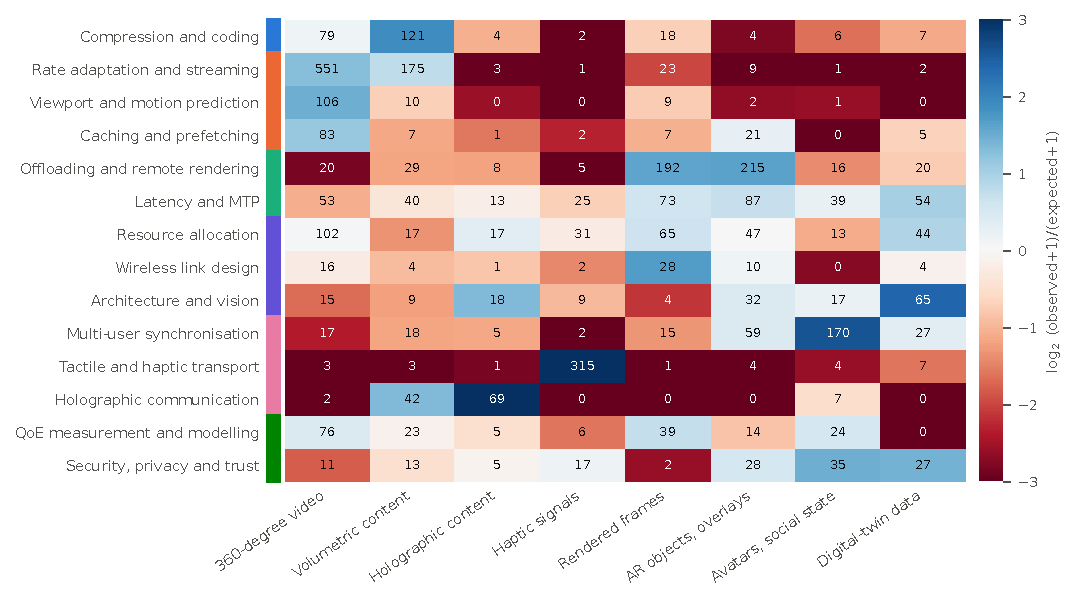
\includegraphics[width=0.86\linewidth]{fig_heatmap}
\caption{Networking problem (rows, grouped by function) against content type (columns). Numbers are
papers. Colour is $\log_2$ of observed over expected counts under independence: blue cells hold more
papers than expected and red cells fewer. ``XR traffic in general'' is omitted.}\label{fig:heatmap}
\end{figure}

\section{What Is Sent: Representing and Encoding Immersive Content}\label{sec:encode}

Every networked XR system must first decide what its content is: a sphere of pixels, a set of camera
views, a cloud of points, the parameters of a learned scene model or a stream of force samples. The
design question is which representation travels and how it is compressed. The choice fixes four
quantities that every later function inherits. The \emph{bitrate floor},
below which quality collapses, sets what the network must supply (\cref{sec:provision}). The
\emph{encoder delay} counts against the interaction budgets of \cref{sec:compute,sec:connect}. The
\emph{decoder cost} lands on a battery-powered headset or phone. \emph{Viewport dependence} decides
whether the stream can be cut to what the user will see, and so whether prediction
(\cref{sec:anticipate}) has anything to act on.

We group representations into four families by what they send (\cref{tab:encode-families}).
\emph{Image-based} representations send what cameras see. \emph{Geometry-based} representations send
the shape of the scene. \emph{Learned} representations send a model of the scene, or its meaning, for
the receiver to regenerate. \emph{Signal-based} representations send a physical signal sampled by the
rules of the sense that receives it. \Cref{fig:encode-chains} follows one chain per family from capture
to display.

\begin{figure}[t]
\centering
\begin{adjustbox}{max width=\linewidth}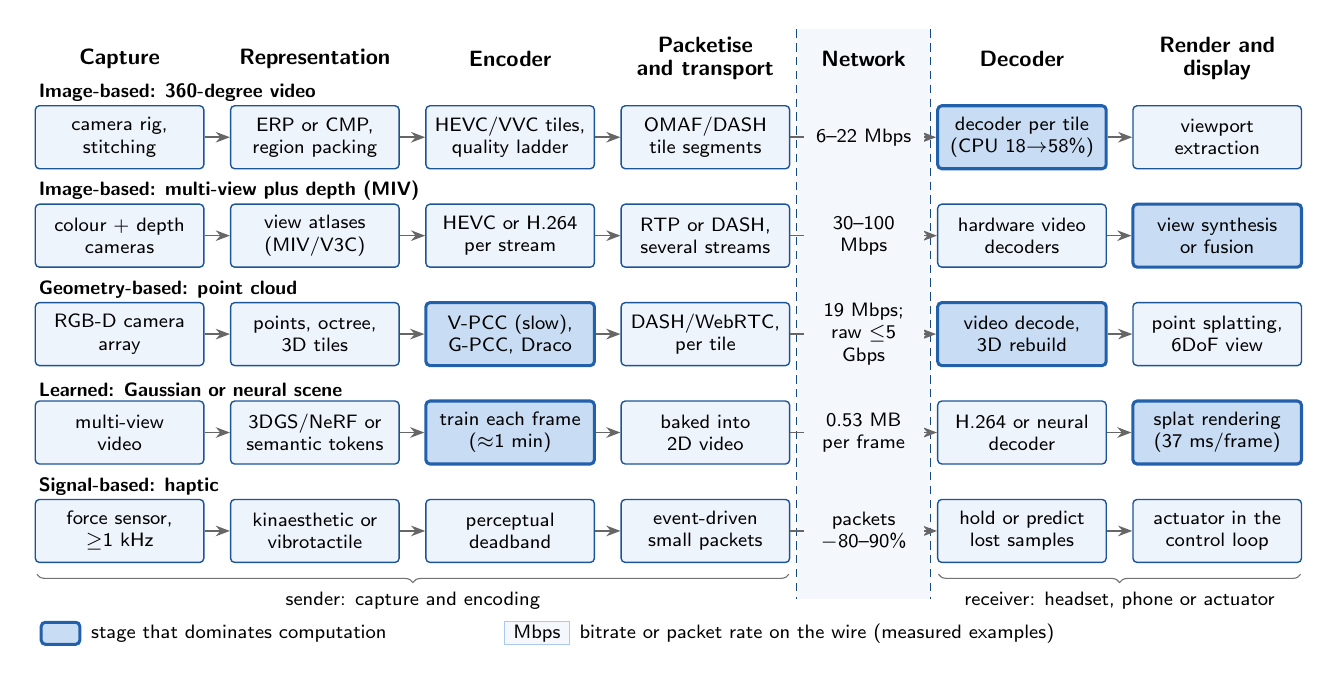
\begin{tikzpicture}[font=\sffamily\scriptsize,
  st/.style={draw=encode!70!black, fill=encode!8, rounded corners=1.5pt, line width=0.5pt,
             text width=2.0cm, minimum height=0.8cm, align=center, inner sep=2pt},
  hv/.style={st, fill=encode!26, draw=encode!80!black, line width=1.1pt},
  flow/.style={-{Stealth[length=1.8mm]}, line width=0.55pt, draw=black!60},
  rate/.style={font=\sffamily\scriptsize, fill=encode!5, inner sep=1pt, align=center, text=black,
               text width=1.45cm},
  hd/.style={font=\sffamily\footnotesize\bfseries, align=center, text width=2.1cm},
  lane/.style={font=\sffamily\scriptsize\bfseries, anchor=south west, inner sep=0.5pt}]
  \def\xa{0} \def\xb{2.48} \def\xc{4.96} \def\xd{7.44} \def\xn{9.45} \def\xe{11.46} \def\xf{13.94}
  % network band
  \fill[encode!5] (8.6,0.62) rectangle (10.3,-6.62);
  \draw[densely dashed, encode!60!black, line width=0.5pt] (8.6,0.62) -- (8.6,-6.62);
  \draw[densely dashed, encode!60!black, line width=0.5pt] (10.3,0.62) -- (10.3,-6.62);
  \node[font=\sffamily\footnotesize\bfseries] at (\xn,0.25) {Network};
  % headers
  \foreach \x/\t in {\xa/Capture, \xb/Representation, \xc/Encoder, \xd/Packetise\\[-1pt]and transport,
                     \xe/Decoder, \xf/Render and\\[-1pt]display}
    \node[hd] at (\x,0.25) {\t};
  % one lane: id, y, name, capture, representation, encoder, transport, encoder style,
  % decoder, decoder style, renderer, renderer style, rate on the wire
  \newcommand{\lanerow}[8]{%
    \node[lane] at (-1.05,#2+0.43) {#3};
    \node[st] (c#1) at (\xa,#2) {#4};
    \node[st] (r#1) at (\xb,#2) {#5};
    \node[#8] (e#1) at (\xc,#2) {#6};
    \node[st] (t#1) at (\xd,#2) {#7};
    \draw[flow] (c#1) -- (r#1); \draw[flow] (r#1) -- (e#1); \draw[flow] (e#1) -- (t#1);
    \lanerest{#1}{#2}}
  \newcommand{\lanerest}[2]{\def\li{#1}\def\ly{#2}\lanerestb}
  \newcommand{\lanerestb}[5]{%
    \node[#2] (d\li) at (\xe,\ly) {#1};
    \node[#4] (p\li) at (\xf,\ly) {#3};
    \draw[flow] (t\li) -- (d\li); \draw[flow] (d\li) -- (p\li);
    \node[rate] at (\xn,\ly) {#5};}
  \lanerow{1}{-0.75}{Image-based: 360-degree video}{camera rig,\\stitching}{ERP or CMP,\\region packing}
    {HEVC/VVC tiles,\\quality ladder}{OMAF/DASH\\tile segments}{st}
    {decoder per tile\\(CPU 18$\to$58\%)}{hv}{viewport\\extraction}{st}{6--22 Mbps}
  \lanerow{2}{-2.0}{Image-based: multi-view plus depth (MIV)}{colour + depth\\cameras}{view atlases\\(MIV/V3C)}
    {HEVC or H.264\\per stream}{RTP or DASH,\\several streams}{st}
    {hardware video\\decoders}{st}{view synthesis\\or fusion}{hv}{30--100\\Mbps}
  \lanerow{3}{-3.25}{Geometry-based: point cloud}{RGB-D camera\\array}{points, octree,\\3D tiles}
    {V-PCC (slow),\\G-PCC, Draco}{DASH/WebRTC,\\per tile}{hv}
    {video decode,\\3D rebuild}{hv}{point splatting,\\6DoF view}{st}{19 Mbps;\\raw $\leq$5 Gbps}
  \lanerow{4}{-4.5}{Learned: Gaussian or neural scene}{multi-view\\video}{3DGS/NeRF or\\semantic tokens}
    {train each frame\\($\approx$1 min)}{baked into\\2D video}{hv}
    {H.264 or neural\\decoder}{st}{splat rendering\\(37 ms/frame)}{hv}{0.53 MB\\per frame}
  \lanerow{5}{-5.75}{Signal-based: haptic}{force sensor,\\$\geq$1 kHz}{kinaesthetic or\\vibrotactile}
    {perceptual\\deadband}{event-driven\\small packets}{st}
    {hold or predict\\lost samples}{st}{actuator in the\\control loop}{st}{packets\\$-$80--90\%}
  % sender / receiver braces
  \draw[decorate, decoration={brace, amplitude=3pt, mirror}, draw=black!55]
    (-1.05,-6.3) -- (8.5,-6.3) node[midway, below=3pt, font=\sffamily\scriptsize] {sender: capture and encoding};
  \draw[decorate, decoration={brace, amplitude=3pt, mirror}, draw=black!55]
    (10.4,-6.3) -- (15.0,-6.3) node[midway, below=3pt, font=\sffamily\scriptsize] {receiver: headset, phone or actuator};
  % legend
  \node[hv, text width=0.35cm, minimum height=0.28cm] (lg) at (-0.75,-7.05) {};
  \node[anchor=west, font=\sffamily\scriptsize] at (lg.east) {stage that dominates computation};
  \node[rate, text width=0.75cm, draw=encode!40] (lr) at (5.3,-7.05) {Mbps};
  \node[anchor=west, font=\sffamily\scriptsize] at (lr.east) {bitrate or packet rate on the wire (measured examples)};
\end{tikzpicture}\end{adjustbox}
\caption{Transmission chains from capture to display for one or two representations of each family. No
chain is cheap at both ends: a low rate on the wire is bought with encoder delay (V-PCC, per-frame
training) or with computation on the receiver (tile decoding, view synthesis, splat rendering). Figures:
360-degree video \cite{W2623027537,W2896840651}, multi-view streams \cite{W4200107448}, point clouds
\cite{W4362496249,W3021314748}, Gaussian video \cite{W4404525293}, deadband coding \cite{W2912555763}.}
\label{fig:encode-chains}
\end{figure}

\begin{table}[t]
\centering\small
\caption{Representation families and where their cost lands. Figures are examples measured on the cited
systems under different conditions; they locate each cost but are not matched operating points.}
\label{tab:encode-families}
\setlength{\tabcolsep}{3pt}
\renewcommand{\arraystretch}{1.08}
\begin{tabularx}{\linewidth}{@{}>{\raggedright\arraybackslash}p{1.6cm}>{\raggedright\arraybackslash}X%
>{\raggedright\arraybackslash}p{2.3cm}>{\raggedright\arraybackslash}p{2.4cm}%
>{\raggedright\arraybackslash}p{2.5cm}>{\raggedright\arraybackslash}p{2.55cm}@{}}
\toprule
Family & Idea & Cost on wire & Cost at sender & Cost at receiver & Maturity\\
\midrule
Image & 360-degree video: sphere projected to rectangles, bits on the viewport & 6--22~Mbps & low; tiles lose 7--10\% efficiency & a decoder per tile, CPU 18$\to$58\% & standard (OMAF), deployed\\
\addlinespace[2pt]
Image & Multi-view plus depth (MIV): camera views, new views synthesised & 30--100~Mbps & low; hardware video encoders & several decoders and view synthesis & standard; rarely tested on networks\\
\addlinespace[2pt]
Geometry & Point clouds (V-PCC, G-PCC, Draco) & 19~Mbps live; raw up to 5~Gbps & V-PCC hours per second of content; G-PCC, Draco fast & 3D rebuild; 30~fps on phones needs inter-frame coding & standard; on-demand prototypes\\
\addlinespace[2pt]
Geometry & Meshes: surfaces from fused depth & 14~Mbps mean (reconstructed scene) & reconstruction & rasterisation & static codecs benchmarked\\
\addlinespace[2pt]
Learned & Neural scene (NeRF, 3DGS): model parameters per frame & 0.53~MB per frame & training $\approx$1~min per frame & splat rendering, 37~ms per frame & research prototypes\\
\addlinespace[2pt]
Learned & Semantic and generative: meaning, not pixels & 93--99.9\% less & inference, shared knowledge base & generative inference; 13.7~s end to end & simulation, one 5G prototype\\
\addlinespace[2pt]
Signal & Haptic: samples sent only above a perceptual threshold & 80--90\% fewer packets & negligible, delay-free & hold or predict missing samples & standard (IEEE~1918.1.1)\\
\addlinespace[2pt]
Signal & Holographic: light field or phase pattern & 6.63~TBps by arithmetic; 173~Mbps measured & V-PCC 11--42~min per second & display not characterised & requirement tables\\
\bottomrule
\end{tabularx}
\end{table}

\subsection{Image-based: send what a camera sees}
Image-based representations keep the 2D video chain and its hardware codecs. Their open questions are
how the scene maps onto rectangles and how many decoders the client can afford.

\emph{Projected 360-degree video} assumes a viewer who turns the head but stays in place (3DoF), and wins
when that holds. Concentrating bits on the viewport saves bitrate, but less than it saves pixels:
Oculus's offset cube used fewer than half the pixels of an equirectangular frame, yet saved only
5.6--16.4\% of bitrate \cite{W2623027537}. The delivery unit is contested. Viewport-specific versions
multiply storage; tiles share one encode but cost 7.3--10.4\% in coding efficiency, and Flare's tile
decoders raised phone CPU load from 18\% to 58\% \cite{W2896840651}. Gaze is the stronger lever.
Gaze-based quantisation saved 40--47\% of bitrate in cloud VR gaming \cite{W3174397927}, and
gaze-contingent compression was five times more effective when motion-to-photon (MTP) latency stayed
below 15~ms \cite{W4214531162}. Foveation is thus a coding gain that \cref{sec:compute} pays for in
latency.

\emph{Multi-view plus depth} sends colour and depth streams and lets the receiver synthesise the view,
giving limited six degrees of freedom (6DoF) with ordinary video codecs. It assumes the receiver can
afford view synthesis, and it wins in live, two-way systems because it needs no slow 3D encoder. Project
Starline sends seven H.265 streams at 30--100~Mbit/s and fuses them at the receiver, because real-time
3D compression was impossible at its resolution \cite{W4200107448}. MPEG Immersive
Video (MIV) standardises this path \cite{W4210296418}, yet no study has streamed MIV to users over a real
network.

\subsection{Geometry-based: send the shape}
Geometry-based representations send the scene itself, so the receiver can render any viewpoint. The
price is weight: raw point clouds need 720~Mbit/s at 200K points and 30~fps \cite{W3021314748}, one to
three orders of magnitude more than 2D video.

Point-cloud codecs trade compression ratio against speed, and the trade is established. V-PCC projects
patches onto planes and reuses video codecs; it reaches lossy ratios of 100--500 but took about 4~hours
to encode 30 frames \cite{W3096788322}. G-PCC and Draco code geometry in 3D, run fast and compress less,
so live systems avoid V-PCC. In VR2Gather, the MPEG Anchor codec cut 281.8 to 19.0~Mbit/s but raised
latency from 40.6 to 278.7~ms, and parallel tiles brought it back to 90.6~ms \cite{W4362496249}: coding,
not transit, set the delay. The receiver is the second constraint: Hermes reached 30~fps on phones only
by exploiting inter-frame correlation \cite{W4387967921}. No codec wins everywhere; in a comparison of
five codecs the best choice depended on content and viewing behaviour \cite{W4321488303}.

Geometry's advantage is a richer viewport dependence: points can be culled by visibility, occlusion and
distance, not only by direction. ViVo saved 40\% of bandwidth at SSIM above 0.99, but only
10\% for phone users \cite{W3021314748}. Meshes are less explored: a reconstructed mesh for robot teleoperation needed
14~Mbit/s on average \cite{W2966611292}.

\subsection{Learned: send a model or a meaning}
Learned representations replace explicit content with something the receiver must regenerate. They
promise the largest savings and move the most work to the two ends.

\emph{Neural scene representations} (NeRF, 3D Gaussian splatting) send model parameters. The most
deployable design reuses existing hardware: V$^3$ bakes dynamic Gaussians into 2D video for H.264
decoders and reaches 32.97~dB PSNR at 0.532~MB per frame and 27~fps on a phone \cite{W4404525293}. At
30~fps that is about 128~Mbit/s, the range of multi-view video, so the gain is rendering freedom rather
than bitrate. Training takes about a minute per frame, which rules out live content, and error control and
quality assessment remain open \cite{W4408847683}.

\emph{Semantic and generative codecs} send meaning and assume that sender and receiver share a knowledge
base or a generative model. Their comparisons are the weakest of any family. WiserVR sent
1.81 instead of 28.3~Mbit for 20 frames, in an AWGN simulation that ignored the cost of sharing the
knowledge base \cite{W4324296656}. The one generative prototype timed end to end cut bandwidth by
99.93\% but raised latency from 980~ms to 13.66~s \cite{W4403677254}. Fidelity metrics differ between
studies and can disagree with perceived realism \cite{W4385452934}, and baselines are usually BPG with
LDPC rather than HEVC or VVC. An order-of-magnitude saving is plausible; its price in inference delay
and energy is assumed rather than measured.

\subsection{Signal-based: send the physical signal}
Signal-based representations code a physical quantity by the limits of the sense that receives it.
Haptic and holographic content sit at opposite ends of the rate scale.

\emph{Haptic signals} need little rate and strict timing. Kinaesthetic samples travel at 1~kHz or more to
keep the control loop stable, and perceptual deadband coding sends a sample only when its change exceeds
a Weber fraction (7--15\% for force), removing 80--90\% of packets without perceptible loss. Two
independent implementations of the IEEE~1918.1.1 codec reproduced the same rates and errors
\cite{W2912555763}, an established result, though for one contact point. Vibrotactile coding is
open-loop and tolerates tens of milliseconds of transform delay \cite{W2911218692}; learned tactile
codecs report 80--92\% cuts, but only against other learned codecs \cite{W7131889935}. Deadband coding
makes traffic bursty, unlike the periodic 1~ms flow that transport studies assume.

\emph{Holographic content} has no agreed representation, so its requirement figures depend on an unstated
one. A light-field display example needs 221~GB per frame, or 6.63~TBps at 30~fps
\cite{W4300960574}. Measured systems used 5--100~Mbps for compressed point clouds over live 5G
\cite{W4312662428} and 173~Mbps for light-field telepresence \cite{W3176472668}: one figure is
uncompressed display arithmetic, the other compressed capture. For live use, codec delay binds first:
V-PCC needs 11--42 minutes to encode one second \cite{W4309030584}.

\paragraph{The choice moves cost; it does not remove it.} No representation is cheap at both ends.
Image-based content is light on the sender and heavy on the wire and the decoders. Geometry cuts the wire
at the price of encoder delay. Learned representations cut it further and move the work into training
and inference. Choosing a representation is choosing where to spend: on the network, the
sender's encoder or the receiver's processor. Nor is the choice independent. Remote rendering
(\cref{sec:compute}) collapses any representation back into 2D video at the edge, trading decoder cost
for MTP latency; viewport dependence bounds what prediction can save (\cref{sec:anticipate}); encoder
delay decides which representations two-way telepresence can use (\cref{sec:connect}). The ratio--speed
trade within each family is established; that new representations win across families is assumed, since
none has been compared with the others at matched quality.

\begin{openproblems}
\item \textbf{Which representation minimises end-to-end cost?} Point clouds, meshes,
  multi-view video and Gaussian splats have never been compared on the same content at matched perceived
  quality. Streaming shared scenes over replayed 5G and Wi-Fi traces would measure rate, encoder
  delay and decoder load.
\item \textbf{Do semantic and generative savings survive latency?} Reported savings come from AWGN
  simulations with weak baselines. Comparing semantic codecs with HEVC, VVC and V-PCC at matched quality
  on a real 5G link, timing inference at both ends, would show whether they suit interactive use.
\item \textbf{How should new representations be judged?} No rating data exist for compressed Gaussian,
  neural or generative reconstructions viewed in a headset, so PSNR and LPIPS are unvalidated for their
  artefacts. A 6DoF rating study across codecs and rates would provide ground truth.
\item \textbf{Can codecs track a mobile link?} Rate control is tuned at fixed rates, and neural codecs lack
  bitrate ladders and loss handling. Rate control driven by measured capacity, judged by frame-deadline
  misses, would test whether codec gains hold on cellular links.
\item \textbf{What does a hologram actually cost to send?} Requirement tables rest on display arithmetic,
  not captured content. Coding one scene as point clouds, splats, light fields and phase holograms and
  recording the traffic would replace assumed figures with measured ones.
\item \textbf{How do coded haptic streams behave under real loss?} Haptic codecs are evaluated on one-off
  recordings with one contact point. Shared multi-point recordings and a user study of deadband and
  vibrotactile codecs over replayed impairments would test perceptual transparency.
\end{openproblems}

\section{Delivering Ahead of the User: Adaptation, Prediction and Caching}\label{sec:anticipate}

An immersive client displays only a fraction of what it could receive, and it must request that fraction before the user looks there. This section asks how a system decides what to fetch, at what quality and from where, ahead of the user's head and body. Three problem cells answer the question. Rate adaptation and adaptive streaming is the largest problem cell in the atlas, with \nxrNProbRateAdaptationStreaming{} papers (\nxrShProbRateAdaptationStreaming{} of the corpus), but its share fell from \nxrShProbRateAdaptationStreamingEarly{} in 2017--2019 to \nxrShProbRateAdaptationStreamingLate{} in 2022--2024: it grew by \nxrCagrProbRateAdaptationStreaming{} a year while the corpus grew by \nxrCagrTotal{}. Viewport and motion prediction (\nxrNProbViewportMotionPrediction{} papers, \nxrCagrProbViewportMotionPrediction{} a year) and caching and prefetching (\nxrNProbCachingPrefetching{} papers, \nxrCagrProbCachingPrefetching{} a year) are smaller and growing faster. The decline mirrors that of 360-degree video, the content all three were built for, whose share fell from \nxrShContVideoThreeSixtyEarly{} to \nxrShContVideoThreeSixtyLate{} over the same periods. Evidence thins along the chain: \nxrRealRateAdaptationStreaming{} of rate-adaptation papers use a real testbed and \nxrUsersRateAdaptationStreaming{} involve users; prediction is judged mainly on recorded traces (\nxrTraceViewportMotionPrediction{}); caching is judged mainly in simulation (\nxrSimCachingPrefetching{}) and never with users. Representations and codecs are treated in \cref{sec:encode}, and remote rendering in \cref{sec:compute}.

\subsection{Viewport-adaptive streaming: spending bits where the user looks}

Tiled delivery of 360-degree video saves bandwidth, and the saving shrinks as the test becomes realistic (\cref{tab:anticipate-savings}). With a scripted viewport and an all-high-quality baseline, hexaface tiling saved up to 72\% \cite{W2524582890}; HEVC tiles saved 65\% for a static viewport and over 40\% with recorded head motion \cite{W2623784065}; Flare, run on phones over commercial LTE, saved 26--35\% \cite{W2896840651}. The saving is paid for twice. Tiling costs coding efficiency, a median 7.3--10.4\% for 1-s tiles \cite{W2896840651} and up to 37.3\% more bitrate for an 8$\times$5 grid at low resolution \cite{W2623784065}. Decoding many tiles costs the client: Flare raised phone CPU load from 18\% to 58\% \cite{W2896840651}, and Rubiks layered its tiles to fit smartphone decoders \cite{W2826107421}. Prediction error is the main limiter, so controllers hedge. 360ProbDASH fetched tiles in proportion to their viewing probability and raised viewport PSNR by about 39\% \cite{W2766324256}, and segments of at most 2--3~s bound the cost of a wrong guess \cite{W2527384707}.

How the controller should be built is contested. Deep reinforcement learning, used by about a quarter of the cell, reports 20--30\% gains over earlier heuristics \cite{W2920378308,W3159074940}; BOLA360, a buffer-based controller with a near-optimality proof and no training, reports 6--110\% \cite{W4394890851}. The two families have never been compared on shared traces, and learned policies degrade on unseen viewing patterns and networks \cite{W4403826584,W4400409717}. Both rest on an assumed objective: a hand-weighted sum of viewport quality, rebuffering and quality switches. No abstract in the cell names an ITU-T QoE model, although tile extensions of P.1203 and P.1204.3 exist \cite{W3200608537,W3168206114}. The quality term is itself disputed: one study favours PSNR \cite{W2741833902}, another VMAF \cite{W3115841380}, and a database of 378 viewport videos found that mainstream models fail for viewport-adaptive streams \cite{W4402916896}. Even delay sensitivity is unsettled. An OMAF analysis found end-to-end delay decisive for tile adaptation \cite{W2914790472}, whereas a subjective test found that 47~ms of delay barely changed ratings \cite{W2949677285}.

Most of this evidence comes from one on-demand client on an emulated link. Live streaming removes the pre-encoded ladder and brings the uplink into the loop. Live360 sets camera upload rates by viewer interest and reports twice the average QoE of its baselines, in its own metric \cite{W4317796966}, while YouTube Live delivered 360-degree streams with 4.2--44.2~s camera-to-display delay depending on mode \cite{W4361857501}. Multicast exploits the similarity of viewers' motion and saved over 50\% \cite{W2725312916}, but adaptation for several headsets behind one bottleneck has reached a testbed in only three papers and users in none \cite{W4377000454,W2890617053}. Wireless access is the largest blind spot. Only two abstracts in the cell use commercial cellular traces \cite{W3021314748,W2810704880}, although mmWave variability and handover already require new mechanisms such as band switching \cite{W3195004621}.

\begin{table}[t]
\centering\small
\caption{Bandwidth saved by viewport- and visibility-adaptive delivery, ordered within each content type from idealised to realistic evaluation. The saving falls as the viewport and the network become real.}
\label{tab:anticipate-savings}
\begin{tabularx}{\linewidth}{@{}lXrl@{}}
\toprule
Content & Condition & Saving & Source\\
\midrule
360-degree & Perfect knowledge of future motion (bound) & 80\% & \cite{W2585813514}\\
360-degree & Scripted viewport, against all tiles at high quality & up to 72\% & \cite{W2524582890}\\
360-degree & HEVC tiles, static viewport / recorded head motion & 65\% / $>$40\% & \cite{W2623784065}\\
360-degree & Predicted motion with redundancy, $<$0.1\% failure & 45\% & \cite{W2585813514}\\
360-degree & Phones on commercial LTE, 4 users, 3 videos & 26--35\% & \cite{W2896840651}\\
Volumetric & Gaze-driven delivery on HoloLens~2 & up to 67\% & \cite{W4399323898}\\
Volumetric & Visibility-aware, commercial 5G, headset / phone users & 40\% / 10\% & \cite{W3021314748}\\
\bottomrule
\end{tabularx}
\end{table}

\subsection{Six degrees of freedom: adapting volumetric scenes}

Volumetric streaming carries the same idea into 6DoF, where the unit of adaptation becomes a 3D cell, an object or a level of detail, and visibility depends on position, distance and occlusion as well as direction. It is the fastest-growing part of rate adaptation, at about forty papers a year by 2025. ViVo combined the three visibility tests and saved 40\% of data on average, and up to 80\%, over commercial 5G at SSIM above 0.99 \cite{W3021314748}. The same content saved 40.0\% for headset users but only 9.98\% for phone users, so the gain depends on how people move. Related designs allocate rate across 3D tiles with a window-based buffer \cite{W2963389850}, solve a QoE-driven knapsack \cite{W4210824758}, keep octrees decodable in parallel on mobile devices \cite{W3088533413}, or refine quality progressively with neural compression \cite{W4392405518}.

No general allocation policy has emerged. PCC-DASH found that the best multi-object strategy depends on the scene and the camera path \cite{W2982262421}, and its subjective follow-up had to test whether objective and subjective rankings even agree \cite{W3036519337}. The field assumes that its navigation traces are representative, yet the newest public set has 15 participants \cite{W4408870156}, and only about one volumetric adaptation paper in thirty evaluates with users. Two-way volumetric communication breaks the buffer-based model altogether. Systems reuse low-latency DASH \cite{W3030878847} or WebRTC \cite{W4394890952}, a tiled user-adaptive point-cloud system needed 14~Mbps instead of about 300~Mbps in a 33-user study \cite{W4304091566}, and LiVo reached a mean opinion score of 4.1 \cite{W4416659451}. In these systems, adaptation is coupled loosely, if at all, to congestion control. Gaussian splatting has layered representations meant for adaptive streaming, but they are judged on visual fidelity rather than on behaviour under variable throughput \cite{W4402704690}.

\subsection{Prediction: how far ahead, and against which baseline}

The prediction horizon couples the two halves of the controller. A deep buffer absorbs throughput dips but forces the system to predict the viewport seconds ahead; a shallow buffer needs only short predictions but stalls when throughput drops. Accuracy falls steeply with horizon: Flare's best predictor reached median accuracies of 90.5\%, 72.9\%, 58.2\% and 35.2\% at 0.2, 0.5, 1 and 3~s \cite{W2896840651}, and a cross-dataset benchmark found no algorithm accurate much beyond 300~ms \cite{W3089527252}. For on-demand content, earlier viewers are the strongest long-horizon signal. Cross-user prediction raised accuracy by 20.2 percentage points \cite{W2896449077}, and adding other users' viewports raised the 1--10~s hit rate from 0.7283 to 0.7791 \cite{W2963428739}. Live content has no such history and relies on online learning or object semantics \cite{W4243538177,W3141438256}. Saliency and gaze help in ablations, more at long horizons \cite{W4387148495,W4387968308}.

Whether deep models beat simple predictors is the central controversy. On the Tsinghua dataset, persistence (keep the current viewport) reached a hit rate of 0.8355, against 0.8402 for a sequence-to-sequence model and 0.8464 for a single LSTM \cite{W2963428739}; for 6DoF pose, simple statistical models performed surprisingly well \cite{W4379805466}. Learned models report large gains mostly over other learned models. A fusion transformer reached an average precision of 0.954 at 1~s against 0.901 for the previous best, but on a random split of sliding windows that placed the same videos and users in training and test \cite{W4387148495}. Its accuracy also had a price, 74~ms per batch on a desktop GPU against 21~ms for a scanpath-only transformer \cite{W4387148495,W4251137679}. Fewer than one prediction paper in ten names a persistence, linear or Kalman baseline, and no evaluation protocol with disjoint videos and users is accepted.

Two further assumptions go untested. Controllers need calibrated uncertainty to size tile margins, yet predictors output point estimates. Predicting the predictor's own deviation saved 45\% of bandwidth at under 0.1\% failure \cite{W2585813514}, and some models output several possible futures \cite{W4280601181}, but no paper the atlas read reports calibration. Second, accuracy is assumed to translate into experience, yet closed-loop tests with real systems fell from 9 of 74 prediction papers in 2016--2022 to 1 of 54 in 2023--2026. Wireless uses of prediction inherit the problem. A federated predictor for mmWave association reduced breaks in presence by up to 16\% and 26\% against centralised baselines, using traces that paired hourly location samples with unrelated head orientations \cite{W2975296300}, whereas a 60~GHz measurement found 3D motion too unpredictable for beam steering \cite{W2791171246}. Pose prediction that hides motion-to-photon (MTP) latency in remote rendering is discussed in \cref{sec:compute}.

\subsection{Caching and prefetching: placing content before it is requested}

Viewport-aware caching beats popularity-only replacement, a result replicated by independent groups but always against weak baselines. Placing tiles by cross-user viewport similarity raised the edge hit ratio by at least 40\% over LFU and 17\% over LRU \cite{W2896595273}. OpCASH covered more than 95\% of the viewport from cache after 24 views and fetched 85\% less data from the origin \cite{W4288370107}; VRCT rebuilt viewports from partly cached tiles, raising hit ratio by 29\% and cutting backhaul by 44\% \cite{W4377008005}; CUBIST combined reactive and proactive caching for an 87\% hit ratio \cite{W3213361583}. For live 360-degree video, predictive edge caching cut backhaul by up to 76\% \cite{W4390136482}. Prefetching extends to AR and volumetric content: world-scale AR retrieval missed 20\% fewer deadlines with ten times fewer wasted bytes \cite{W4379932440}, and PACE raised modelled QoE by up to 54.8\% \cite{W4415047817}. Joint designs that cache and also transcode, render or synthesise views at the edge report lower latency in simulation \cite{W2979447669,W4210795263}, a result that holds almost by construction, because the joint problem contains the decoupled one.

Three questions remain open. The first is granularity: fixed tiles, variable tiles that rarely recur \cite{W4288370107}, or similarity caching over continuous orientations \cite{W3156984197}, never compared head to head. The second is the interaction with adaptation: cache hits distort the throughput estimates that DASH clients rely on \cite{W3122351391}, yet most caching papers assume an ideal client. The third is whether multi-agent and graph learners add anything beyond good viewport prediction, which cannot be settled while XRFlux remains the only shared benchmark \cite{W4409763640}. Wireless caching sharpens the gap between theory and practice. Multi-antenna coded caching promises 100--400\% more parallel streams, but its authors list subpacketisation and synchronised requests as obstacles \cite{W4381251523}, and a learned UAV small-cell cache was tested with 20 simulated users \cite{W2962896865}. The common assumption is that hit ratio stands for experience. No caching scheme in the atlas has been evaluated with users, and fewer than one caching paper in twenty addresses 6DoF content, which is reusable across viewpoints and users.

\begin{openproblems}
\item \textbf{Prediction and adaptation are not validated in closed loop with users.} Real-system tests of predictors fell to 1 of 54 papers after 2022, and ABR objectives are hand-weighted. A tiled player that runs persistence, Kalman and learned predictors under ABR policies over real bandwidth, with a within-subjects rating study, would show whether accuracy rankings survive.
\item \textbf{No dataset joins head motion, network conditions and ratings from the same session.} Four dataset papers pair head data with network traces and four with ratings; replay removes the viewer's reaction to quality. Live sessions over Wi-Fi and commercial 5G, logging pose, packets and continuous ratings, would close this gap.
\item \textbf{Adaptation over real wireless access is under-evaluated.} The cell has half the expected 5G papers and two abstracts with commercial cellular traces. Paired head-motion and radio traces from walking and seated users, replayed in emulation and run live, would test whether PHY and MAC hints reduce stalls.
\item \textbf{6DoF adaptation and caching lack user-validated QoE and realistic navigation traces.} Volumetric streaming grows fastest, yet trace sets have about 15 participants and volumetric caching is almost unstudied. Larger 6DoF traces, paired comparisons of rendered views and a level-of-detail edge cache shared by co-located users are needed.
\item \textbf{Caching gains have never been shown to users or outside simulation.} No caching paper has users, and none of the coded, D2D or UAV caching papers uses traces or a testbed. An unmodified HTTP edge cache serving tiled DASH, comparing LRU, viewport-aware and Belady policies with viewers, would quantify perceptible benefit.
\item \textbf{Motion-driven wireless decisions use mismatched position and orientation traces.} Seven of nine such papers are simulations, and the one measurement found motion too unpredictable for 60~GHz beam steering. Room-scale multi-user sessions recording 6DoF tracking with synchronised link measurements would show how far ahead blockage is predictable.
\end{openproblems}

\section{Where Computation Happens: Offloading, Remote Rendering and Latency}\label{sec:compute}

A headset has a few watts of power and a few milliseconds of slack. This section asks which stages of
the sense--render--display pipeline should run on the device, at the edge or in the cloud, and how the
delay that each split adds is budgeted, measured and hidden. The function holds \fnComputeN{} papers,
\fnComputeSh{} of the corpus, and its share has held steady (\fnComputeEarly{} in 2017--2019,
\fnComputeLate{} in 2022--2024). It joins four cells: offloading and remote rendering
(\nxrNProbOffloadingRemoteRendering{} papers), latency (\nxrNProbLatency{}, growing
\nxrCagrProbLatency{} a year against \nxrCagrTotal{} for the corpus), rendered frames
(\nxrNContRenderedFrames{}, whose share rose from \nxrShContRenderedFramesEarly{} to
\nxrShContRenderedFramesLate{}) and AR objects and overlays (\nxrNContArObjectsOverlays{}, whose share
fell from \nxrShContArObjectsOverlaysEarly{} to \nxrShContArObjectsOverlaysLate{}). The evidence is
uneven. Offloading papers divide between real testbeds (\nxrRealOffloadingRemoteRendering{}) and
simulation (\nxrSimOffloadingRemoteRendering{}), and only \nxrUsersOffloadingRemoteRendering{} involve
users. Latency papers are more empirical (\nxrRealLatency{} real testbed, \nxrUsersLatency{} with
users). Radio scheduling and transport are treated in \cref{sec:provision}, and QoE models in
\cref{sec:assure}.

\begin{figure}[t]
\centering
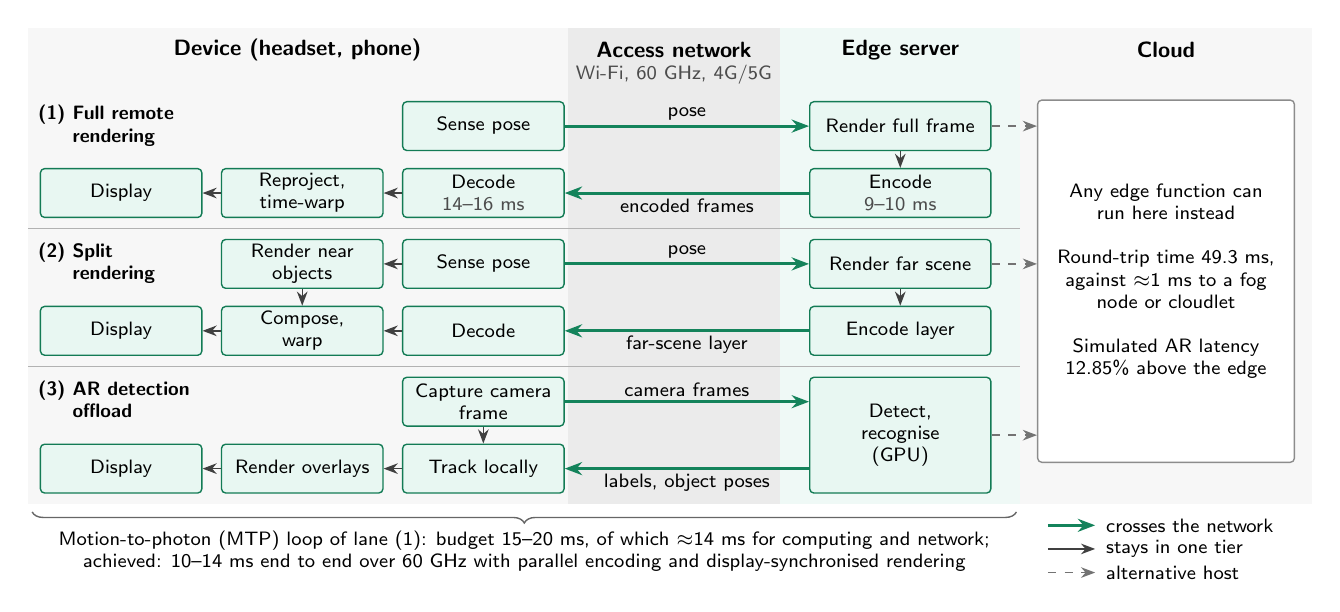
\begin{tikzpicture}[x=1cm, y=1cm, font=\sffamily\scriptsize,
  st/.style={draw=compute!70!black, fill=compute!10, rounded corners=1.5pt, line width=0.5pt,
             minimum width=2.05cm, minimum height=0.62cm, align=center, inner sep=1.5pt},
  est/.style={st, minimum width=2.3cm},
  loc/.style={-{Stealth[length=1.8mm]}, line width=0.5pt, draw=black!75},
  net/.style={-{Stealth[length=2.2mm]}, line width=1.1pt, draw=compute!75!black},
  alt/.style={-{Stealth[length=1.8mm]}, line width=0.5pt, dashed, draw=black!55},
  lab/.style={font=\sffamily\scriptsize, text=black, inner sep=1.5pt},
  lane/.style={font=\sffamily\scriptsize\bfseries, anchor=west, align=left, inner sep=0pt, text=black},
  hdr/.style={font=\sffamily\footnotesize\bfseries, text=black}]
  % ---- tier columns
  \fill[black!3]   (0,-5.65) rectangle (6.85,0.4);
  \fill[black!8]   (6.85,-5.65) rectangle (9.55,0.4);
  \fill[compute!7] (9.55,-5.65) rectangle (12.6,0.4);
  \fill[black!3]   (12.6,-5.65) rectangle (16.3,0.4);
  \node[hdr] at (3.42,0.12)   {Device (headset, phone)};
  \node[hdr] at (8.2,0.12)    {Access network};
  \node[hdr] at (11.075,0.12) {Edge server};
  \node[hdr] at (14.45,0.12)  {Cloud};
  \node[lab, text=black!70] at (8.2,-0.2) {Wi-Fi, 60~GHz, 4G/5G};
  \foreach \y in {-2.15,-3.9} \draw[black!30, line width=0.4pt] (0,\y) -- (12.6,\y);
  % ---- lane 1: full remote rendering
  \node[lane] at (0.12,-0.85) {(1) Full remote\\\phantom{(1) }rendering};
  \node[st]  (s1) at (5.78,-0.85) {Sense pose};
  \node[st]  (d1) at (5.78,-1.70) {Decode\\\textcolor{black!70}{14--16~ms}};
  \node[st]  (w1) at (3.48,-1.70) {Reproject,\\time-warp};
  \node[st]  (p1) at (1.18,-1.70) {Display};
  \node[est] (r1) at (11.075,-0.85) {Render full frame};
  \node[est] (e1) at (11.075,-1.70) {Encode\\\textcolor{black!70}{9--10~ms}};
  \draw[net] (s1) -- node[lab, above] {pose} (r1);
  \draw[loc] (r1) -- (e1);
  \draw[net] (e1) -- node[lab, below] {encoded frames} (d1);
  \draw[loc] (d1) -- (w1); \draw[loc] (w1) -- (p1);
  % ---- lane 2: split rendering
  \node[lane] at (0.12,-2.60) {(2) Split\\\phantom{(2) }rendering};
  \node[st]  (s2) at (5.78,-2.60) {Sense pose};
  \node[st]  (n2) at (3.48,-2.60) {Render near\\objects};
  \node[st]  (d2) at (5.78,-3.45) {Decode};
  \node[st]  (w2) at (3.48,-3.45) {Compose,\\warp};
  \node[st]  (p2) at (1.18,-3.45) {Display};
  \node[est] (r2) at (11.075,-2.60) {Render far scene};
  \node[est] (e2) at (11.075,-3.45) {Encode layer};
  \draw[net] (s2) -- node[lab, above] {pose} (r2);
  \draw[loc] (s2) -- (n2); \draw[loc] (n2) -- (w2);
  \draw[loc] (r2) -- (e2);
  \draw[net] (e2) -- node[lab, below] {far-scene layer} (d2);
  \draw[loc] (d2) -- (w2); \draw[loc] (w2) -- (p2);
  % ---- lane 3: AR detection offload
  \node[lane] at (0.12,-4.35) {(3) AR detection\\\phantom{(3) }offload};
  \node[st]  (s3) at (5.78,-4.35) {Capture camera\\frame};
  \node[st]  (t3) at (5.78,-5.20) {Track locally};
  \node[st]  (o3) at (3.48,-5.20) {Render overlays};
  \node[st]  (p3) at (1.18,-5.20) {Display};
  \node[est, minimum height=1.47cm] (x3) at (11.075,-4.775) {Detect,\\recognise\\(GPU)};
  \draw[net] (s3) -- node[lab, above] {camera frames} (s3 -| x3.west);
  \draw[net] (t3 -| x3.west) -- node[lab, below] {labels, object poses} (t3);
  \draw[loc] (s3) -- (t3); \draw[loc] (t3) -- (o3); \draw[loc] (o3) -- (p3);
  % ---- cloud
  \node[draw=black!45, fill=white, rounded corners=1.5pt, line width=0.5pt, text width=3.05cm,
        minimum height=4.6cm, align=center, inner sep=3pt] (cl) at (14.45,-2.82)
        {Any edge function can\\run here instead\\[8pt]
         Round-trip time 49.3~ms,\\against $\approx$1~ms to a fog\\node or cloudlet\\[8pt]
         Simulated AR latency\\12.85\% above the edge};
  \draw[alt] (r1.east) -- (r1.east -| cl.west);
  \draw[alt] (r2.east) -- (r2.east -| cl.west);
  \draw[alt] (x3.east) -- (x3.east -| cl.west);
  % ---- MTP brace and legend
  \draw[decorate, decoration={brace, mirror, amplitude=4pt}, draw=black!60, line width=0.5pt]
    (0.05,-5.75) -- (12.55,-5.75)
    node[midway, below=5pt, lab, align=center]
    {Motion-to-photon (MTP) loop of lane (1): budget 15--20~ms, of which $\approx$14~ms for computing and network;\\
     achieved: 10--14~ms end to end over 60~GHz with parallel encoding and display-synchronised rendering};
  \begin{scope}[shift={(12.95,-5.92)}]
    \draw[net] (0,0) -- (0.6,0);         \node[lab, anchor=west] at (0.68,0)     {crosses the network};
    \draw[loc] (0,-0.3) -- (0.6,-0.3);   \node[lab, anchor=west] at (0.68,-0.3)  {stays in one tier};
    \draw[alt] (0,-0.6) -- (0.6,-0.6);   \node[lab, anchor=west] at (0.68,-0.6)  {alternative host};
  \end{scope}
\end{tikzpicture}
\caption{Offloading architecture: where each stage runs in full remote rendering, split rendering and
AR detection offload. Each split is the point at which the pipeline crosses the access network;
display, and in AR also tracking, stay on the device in every design. Values: MTP budget \cite{W2784711283}, 60~GHz end-to-end latency
\cite{W2838572662}, encode and phone decode times \cite{W2940859338}, round-trip times
\cite{W2805833065}, simulated edge advantage \cite{W2894645340}.}
\label{fig:compute-pipeline}
\end{figure}

\subsection{Choosing the split}

Proximity is the one placement result that holds across methods. In a shipyard deployment, a fog
gateway and a cloudlet both answered in about 1~ms, against 49.3~ms for a remote cloud; at 240
clients the fog gateway was four times slower than the cloudlet, and the Wi-Fi hop was excluded by
design \cite{W2805833065}. A simulation found that edge execution cut AR latency by 41.44\% against
local and 12.85\% against cloud execution \cite{W2894645340}. What leaves the device varies
(\cref{fig:compute-pipeline}). VR systems render remotely and stream frames. Split designs render near
or interactive objects on the device and the rest remotely; one used 20--30\% of the bandwidth of full
remote rendering and tolerated delays of up to 200~ms \cite{W4399444696,W4389296467,W3080913128}. AR
systems offload perception and render locally. Neural scenes reopen the question: current systems
stream pixels \cite{W4415672032}, dynamic Gaussians \cite{W7106240991} or intermediate level-of-detail
results \cite{W7117245976}, each against its own baseline.

Shared edges add contention, and here the evidence thins. Once many users offload, queueing at the
edge server dominates \cite{W4213053765,W4399320016}, yet schedulers for concurrent rendering sessions
on one GPU exist only in simulation \cite{W3214338661,W4285254743}. The largest strand formulates
offloading as joint computation--communication optimisation, solved by deep reinforcement learning
\cite{W3120265095} or Lyapunov control \cite{W4392567309}. More than nine in ten learning-based
controllers are evaluated only in simulation, and their inputs are assumed: a 2018 YOLO accuracy fit
\cite{W2790412025} reappears in later formulations \cite{W4386702674,W4388068949}, and VR streams are
modelled at a constant 25.32~Mbps \cite{W2596760110}.

Device energy, the main reason to offload, is contested. Models promise savings of 63\%
\cite{W2608841173} and 85\% \cite{W4388068949}. Measurements disagree. Edge offloading halved
smartphone energy for AR on average \cite{W2983318720}, and an edge VR testbed lowered client power
\cite{W4296339041}. A Quest Pro, however, drained its battery 15\% faster with wireless offloading
than with local rendering \cite{W4362489903}, and Air Link on a Quest~2 also cost more energy
\cite{W4387913063}. DeepDecision measured about 2900~mW for offloading regardless of bitrate and frame
rate \cite{W2792220137}, against models that scale energy with transmitted data. Radio tail, decoder
and display power, omitted from most models, are the likely cause.

\subsection{Remote rendering: frames, codecs and pacing}

Compression is mandatory, and its cost is set by pipelining and timing more than by link rate. Raw
stereo frames at 2160$\times$1200 and 90~Hz need 5.6~Gbps. Cutting the Cord split each eye's frame
across four parallel H.264 encoders and aligned rendering with the client's display refresh; over
802.11ad it reached 10--14~ms end to end, against a sequential median above 26~ms, and cut missed
refreshes from 5.3--14.3\% to 0.1--0.2\% \cite{W2838572662}. Phones are tighter. Furion measured
9--10~ms to encode and 14--16~ms to decode H.264 frames, and 27\% of the phone's CPU spent on packet
processing at 400~Mbps \cite{W2940859338}. Removing memory copies brought OpenUVR to 14.32~ms
\cite{W3124215200}.

The renderer knows what the encoder must otherwise estimate, and using it pays. Object-aware
quantisation with gaze saved 40--47\% bandwidth in a subjective test \cite{W3174397927}. Foveated
shading alone did not reduce bitrate, while foveated post-processing or encoding did
\cite{W3186601312}. Other systems change what is streamed: colour plus depth for client-side warping
\cite{W2751899584}, object-space shading atlases \cite{W2903169695}, one eye rendered remotely and the
other reprojected with 36\% lower MTP \cite{W4391557896}, and pixel reuse across frames with 95\% less
frame data \cite{W2928088097}. Each uses its own baseline, so they cannot be ranked (\cref{sec:encode}).
Two assumptions remain untested. No corpus paper measures AV1 or VVC latency for rendered frames;
the only mention is a position paper \cite{W4391267710}. Frame sizes are bursty even under constant-bitrate coding \cite{W4379468406}, and
on one headset the 3GPP traffic model underestimated effective bitrate by 25\% \cite{W4399340506}.

\subsection{AR offloading: stale results and the uplink}

AR offloading succeeds only if the device hides the staleness of remote results. The replicated
design runs a light tracker on the device between remote detections. In one system, without
tracking, 16.7~ms of offload latency raised false detections from 0 to 31.56\%; with tracking and
region-of-interest encoding, offload latency fell from 34.56 to 17.23~ms on 2.4~GHz Wi-Fi
\cite{W2965289829}. CloudAR held 30 frames per second with at least 97\% recognition accuracy
\cite{W2765872303}, Jaguar reached about 33~ms end to end \cite{W2896416526}, and the pattern holds on
HoloLens \cite{W4282961825}. Once the server has a GPU, the network dominates: sending frames as H.264
video rather than images delivered about ten times more frames at 100~kbps \cite{W2792220137}.

The uplink is the bottleneck. In multi-user AR over LTE, median end-to-end latency was 12.5~s, the
radio access network contributed 31.2\%, and uplink bursts triggered TCP slow starts
\cite{W3047439371}. A 5G mmWave measurement found the uplink insufficient for baseline edge detection
\cite{W4390905995}, while vision papers assume 5G solves the problem \cite{W3133913697}. Result sharing among co-located users cut
latency by up to 130$\times$ \cite{W4213053765}, but the overlap it relies on has never been measured. Targets are
contested: below 20~ms \cite{W2609285553}, 50~ms \cite{W3133913697} and 100~ms
\cite{W2898344194,W4282961825} are all quoted. The right one depends on whether overlays are
world-locked and tracked locally, and no study maps network delay to registration error.

\subsection{Budgeting, measuring and hiding delay}

Latency budgets are inherited rather than derived. The common figure is 15--20~ms MTP, leaving about
14~ms for computing and communication \cite{W2784711283}; others assume 13~ms \cite{W2561715836} or
5~ms \cite{W3048503162}. Users are more tolerant once reprojection is active. CloudVR users did not
notice 20~ms of added network latency \cite{W2896076858}, and ALVR users hardly noticed round-trip
times up to 90~ms \cite{W3095344018}, whereas CloudXR quality fell from 75~ms \cite{W4402156718}. In a
crane simulator, display delays of 0--30~ms mattered while controller delay mattered only at 800~ms
\cite{W3086540722}. A budget therefore depends on which loop is meant and how delay is hidden, and
offloading papers rarely state either. Measurement is cheap but rare: a photosensor rig
\cite{W2890615649} and a phone-camera method with under 10~ms uncertainty \cite{W3012329178} measure
MTP directly, yet fewer than one in twenty latency papers report jitter or tail latency.

Latency hiding is the established success. Post-render warping removed up to 80\% of the aiming
penalty of 80~ms added latency \cite{W3089399051}. Rendering beyond the field of view, sized to the
current latency, reduced delivery latency by about 22\% in a simulation with real user data
\cite{W3161249521}. Motion predictors trained on more than 840,000 samples let the edge pre-render
frames \cite{W3094082851}. Reprojection has moved from rotation to translation \cite{W4408848620}, and
selective time-warp leaves head-locked layers untouched \cite{W2908115098}. Stalls of up to four frames
at 90~Hz went unnoticed, and reprojection helped from eight frames upward \cite{W4301184864}. Each
method, however, is tested on its own motion data and with fixed delays, so the gains cannot be
compared.

\begin{openproblems}
\item \textbf{Learning-based offloading controllers are untested on real traces.} More than nine in
  ten are evaluated in simulation with synthetic task sizes and channels. An open benchmark replaying
  measured render times, head motion and 5G/Wi-Fi traces under 3GPP XR traffic would show which gains
  survive.
\item \textbf{Device energy savings are modelled, not measured.} One Quest Pro drained 15\% faster
  with offloading \cite{W4362489903}; one edge testbed lowered power \cite{W4296339041}. Component-level
  measurements of local and remote rendering across headsets, codecs and links would settle the
  direction.
\item \textbf{3GPP XR traffic models go unused and unvalidated.} No offloading paper evaluates against
  them, and the one empirical check found a 25\% bitrate underestimate \cite{W4399340506}. Commercial
  split-rendering traces fitted against the models are needed.
\item \textbf{Rendered-frame streams lack error resilience.} Users rank loss above delay
  \cite{W3095344018,W4404916373}, yet forward error correction, intra refresh and concealment for
  remote rendering barely appear in the corpus. A loss-trace study with user ratings would close this.
\item \textbf{No benchmark couples motion traces, network traces and MTP ground truth.} Warping and
  prediction methods each use their own data and fixed delays. A shared dataset with photodiode MTP
  would let them be ranked.
\item \textbf{The AR camera uplink is unstudied at multi-user scale.} Real-network evidence is
  single-user and pessimistic \cite{W4390905995,W3047439371}. A 5G testbed scheduling several AR
  uplinks in one cell would test whether edge AR scales.
\end{openproblems}

\section{Provisioning the Network: Radio, Resources, Transport and Architecture}\label{sec:provision}

This section asks how access networks, schedulers, transport protocols and system architectures supply
the rate, delay and reliability that XR needs. Three cells hold the work: resource allocation
(\nxrNProbResourceAllocation{} papers, \nxrShProbResourceAllocation{} of the corpus), architecture and
vision (\nxrNProbArchitectureVision{}) and wireless link design (\nxrNProbWirelessLinkDesign{}).
Resource allocation is the second-largest problem cell and the fastest-growing large one: its share rose
from \nxrShProbResourceAllocationEarly{} in 2017--19 to \nxrShProbResourceAllocationLate{} in 2022--24.
Over the same periods the share of papers built on 6G rose from \nxrShTechSixGBeyondFiveGEarly{} to
\nxrShTechSixGBeyondFiveGLate{}. The three cells differ sharply in how they are evaluated.
\nxrSimResourceAllocation{} of allocation papers are simulations and \nxrRealResourceAllocation{} use a
real testbed; \nxrNoEvalArchitectureVision{} of architecture papers have no evaluation at all. Link
design is the most empirical of the three (\nxrRealWirelessLinkDesign{} real testbeds), but no paper in
any of the three cells asked users what they perceived. The argument of this section is that provisioning
research has solved well-posed optimisation problems whose inputs (QoE functions, rendering costs,
traffic and requirement figures) were assumed rather than measured. Offloading decisions are treated in
\cref{sec:compute}.

\subsection{Allocating radio, compute and money}
The design question is how to divide spectrum, power, edge GPU time and caches among XR users so that
each meets a delay or quality target. The established result is that these resources substitute for each
other. Caching rendered fields of view and computing on the device can stand in for bandwidth
\cite{W2887223659,W2945507395}, and joint uplink, downlink and edge allocation saves mobile energy in
collaborative AR compared with offloading each task on its own \cite{W2608841173}. Shared content
adds a second lever. Multicasting overlapping 360-degree viewports over mmWave raised HD delivery by
40--50\% and cut 99th-percentile delay by 17--37\% against unicast, in simulation driven by 50 real head
traces \cite{W2901851646}; the gain shrinks as viewports diverge, so it is unproven for interactive
6DoF content.

What is contested is the objective. The cell optimises at least four incompatible QoE constructs: a
utility of tracking, processing and transmission delay \cite{W2596760110}, regressions of SSIM and VMAF
\cite{W3214250514}, an attention-weighted ``Meta-Immersion'' score \cite{W4379382423} and weighted sums of
quality, delay and variation \cite{W4312555471}. Reported gains of 20--37\% are measured in each paper's
own metric and cannot be compared. Of the \nxrSynXRAQoEN{} allocation papers that optimise QoE, none was
evaluated with users. The second dispute is method. Reinforcement-learning schedulers beat greedy,
random and proportional-fair baselines \cite{W2596760110,W4381946597}, while optimisation papers reach
near-optimal decisions four orders of magnitude faster than a commercial solver \cite{W4324125331}; the
two camps rarely meet on the same traces.

Much of the rest is assumed. Rendering capacity is a free variable in joint radio--rendering allocation
\cite{W4379382423}; the only measured GPU figure is economic, a 4~GB vGPU slice that halved cloud-XR
hourly cost while holding MOS at 4.38 or above \cite{W7115818680}. Metaverse resource markets are the
extreme case. A learned double Dutch auction reached social welfare within about 5\% of the optimum
\cite{W3214250514}, and function sharing raised slice admission revenue by up to 80\% \cite{W4381946597},
but every auction, contract and incentive scheme in the cell uses synthetic valuations and arrivals.
Standards-aligned work is more realistic about traffic. It uses 3GPP XR models and PDU-set quality of
service \cite{W4410582180}, and a delay-tracking PDU-set scheduler served 4--5 times more satisfied users
than PDU-set-aware baselines under scarce resources \cite{W7168254691}. Yet only \nxrSynXRARLStdN{} of
the \nxrSynXRARLN{} reinforcement-learning allocators use these models. The few testbed studies temper
the simulated claims. On an O-RAN testbed, latency-estimation control met 10--16.67~ms targets but
over-provisioned, while packet-size prediction saved resources and lost latency control
\cite{W4410491869}; a latency-steering xApp freed 15.8\% more resources than an equivalent static slice
\cite{W4392175446}.

\subsection{The last hop: directional links, Wi-Fi and 5G}
The link question is how to keep a multi-gigabit, low-delay channel to a moving head. The cell agrees on
the diagnosis: the tail, not the peak rate, limits XR over directional links. Analysis of THz links gives
99.999\% reliability at 20~ms with guaranteed line of sight, but with blockage reliability falls to
68\% at 10~ms and 96\% at 20~ms, and tail delays reach 30--90~ms while the mean stays below 20~ms
\cite{W3022996137}. At 60~GHz, 3D head motion defeated beam search designed for 2D \cite{W2791171246},
and commercial hardware lost up to 4.72\% of packets under 45$^\circ$/s rotation \cite{W4401507876}.
Spatial diversity is the remedy that holds across studies. Dual-beam reception with coordinated access
points raised reliability by up to 22.8\% on real headset motion \cite{W4409076649}, distributed antennas
kept 12~Gb/s under full rotation \cite{W4413277491}, and steering beams from the headset's pose helps
\cite{W4313170175}: predictive beams from a neural radio field halved beam-search error on a 28~GHz array
\cite{W7204893690}.

On Wi-Fi and 5G the bound is medium access, not physical rate. With frames aligned to the 802.11ad beacon
interval, eight headsets at 400~Mbit/s met a 1~ms bound \cite{W3081368317}. Wi-Fi~7 multi-link operation
served 7 rather than 6 AR stations at 80~MHz, and an uninformed greedy policy matched congestion-aware
ones \cite{W4376480829}. Whether downlink or uplink binds is contested, and depends on the assumed rates
\cite{W4376480829,W4409221564}; on real hardware, uplink OFDMA with three headsets disrupted tracking
\cite{W4396853623}. 5G-Advanced link adaptation reports up to 67\% more satisfied XR users
\cite{W4315777456}, entirely from system-level simulation. Two technologies rest on assumption alone.
RIS-assisted XR has never run on hardware, and RIS optimisers that take seconds per slot
\cite{W4318586163} must react within a head rotation \cite{W3207401133}. No XR traffic has crossed a THz
link: the THz analyses assume Poisson arrivals and fixed-size frames \cite{W3022996137}.

\subsection{Transport over shared bottlenecks}
Transport decides what reaches the headset when the bottleneck is shared and lossy. Its share of the
corpus fell from \nxrShTechInternetTransportWebEarly{} to \nxrShTechInternetTransportWebLate{} as
delivery moved from buffered streaming to interactive rendering, although interactive traffic is less
able to absorb loss. Users confirm the risk. In cloud VR, RTT up to 90~ms was hardly noticed while loss
of up to 8\% mattered \cite{W3095344018}; with CloudXR, QoE fell at RTT of 75~ms or more or loss above
6\% (N=30) \cite{W4402156718}; with Air Link, loss raised cybersickness more than delay did (N=16)
\cite{W4404916373}. Despite this, only \nxrSynXRendFECN{} remote-rendering papers address forward error
correction or error resilience \cite{W4399340506,W4409129991}.

Congestion control for XR is nascent. L4S, designed for this traffic, appears in \nxrSynXLFourSN{}
corpus papers. An L4S pipeline for volumetric conferencing converged 45\% faster than Google congestion
control and lost no frames where WebRTC lost 3\% \cite{W4408870658}, and L4S has been carried over 5G for
split rendering \cite{W4401507827}; both studies used controlled bottlenecks with one competing scheme.
Practice has moved ahead of research. Steam Link carries video and control in one QUIC tunnel
\cite{W7160626692}, and WebRTC selective forwarding adapted 13--36\% faster than TCP for volumetric
streams in emulation \cite{W7151958829}. No paper has compared delay-based, loss-based and L4S
controllers with forward error correction on real cellular or Wi-Fi bottlenecks with cross traffic.

\subsection{Architectures and the figures they carry}
Architecture papers propose where functions sit (device, edge, cloud, ledger) and state what the network
must deliver. They agree on the qualitative list (high rate, low delay, reliability, concurrency,
interoperability) and on edge computing as a necessary tier \cite{W4312940001,W4315497913,W4391305431}.
The quantitative figures are where they fail. \Cref{tab:provision-requirements} sets stated
requirements against measured or derived figures; for rates the gap spans two to five orders of
magnitude. The cause is not error in either source but unstated operating points: an uncompressed light
field is not a compressed point cloud, and 360-degree video is not avatar state.

\begin{table}[t]
\centering\small
\caption{Stated requirements against measured or derived figures. The gaps follow from unstated content
representation, codec and control loop.}
\label{tab:provision-requirements}
\begin{tabularx}{\linewidth}{@{}p{2.3cm}XX@{}}
\toprule
Quantity & Stated & Measured or derived \\
\midrule
Per-user metaverse rate & 100--250~Mbps \cite{W4313291084,W4312940001}; $\sim$10$^3\times$ 5G
  throughput \cite{W4391305431} & Horizon Workrooms 2--3~Mbps down, 0.6~Mbps up, +0.5~Mbps per extra
  user (2--5 users) \cite{W4294643390} \\
Holographic call & 1--10~Tbps; 6.63~TBps for a light-field display \cite{W4300960574} & 5--100~Mbps
  for a compressed point cloud over live 5G \cite{W4312662428}; $<$0.2~Mbps for a driven avatar
  \cite{W7123904049} \\
Untethered VR link & 15.75--26.25~Gbps uncompressed \cite{W4401507876} & 400~Mbit/s per 4K headset,
  eight per 802.11ad AP \cite{W3081368317} \\
Cloud VR bitrate & 3GPP XR traffic model & 25\% higher effective bitrate on a Pico Neo~2
  \cite{W4399340506} \\
Interaction latency & 1~ms in \nxrSynOneMsN{} abstracts, \nxrSynOneMsUsersN{} with users & Haptic
  users tolerated 200~ms with adaptive control \cite{W4200154132}; cloud VR RTT up to 90~ms hardly
  noticed \cite{W3095344018} \\
Discomfort threshold & 30~ms \cite{W4313291084} vs $<$20~ms \cite{W4315497913} & Not derived from a
  user study in either source \\
\bottomrule
\end{tabularx}
\end{table}

The figures propagate. One survey reproduces another's requirement table with a reliability target
changed from $1-10^{-6}$ to $1-10^{-5}$ \cite{W4390204075,W4312940001}, and its research agenda reproduces
a third \cite{W4224330100}; fewer than one survey in twenty in the cell reports a search protocol. The
apparent consensus is partly one source counted several times. Measured platforms tell a different story:
throughput, latency and device load on five social VR platforms grew almost linearly with users, because
servers forward avatar data directly \cite{W4307020344,W4294643390}. The scaling bottleneck is server
logic, not access capacity, which weakens the case that 5G cannot carry the metaverse.

Two architectural claims are untested. Blockchain is placed in the interactive data path for ownership
and trust \cite{W4224330100,W4312940001}; \nxrSynXArchChainN{} architecture papers include a ledger,
\nxrSynXArchChainNoEval{} of them without any evaluation, and none has measured the delay it adds, although one concedes that replication raises delay with users
\cite{W4320717855}. Network slicing for XR, by contrast, has testbed evidence: AR, cloud gaming and video
calls were measured under RAN-slice configurations on an O-RAN 5G network \cite{W4386887692}. 6G visions
rarely map their functions onto the 5G-Advanced XR mechanisms that already exist
\cite{W4387933382,W4376607343}, so what 6G must add remains unstated.

\begin{openproblems}
\item \textbf{Allocation objectives are not validated with users.} None of the \nxrSynXRAQoEN{}
  QoE-driven allocators and no link design was evaluated with participants. A QoE-in-the-loop slicing
  study on an open 5G testbed, comparing static, latency-target and QoE-model control with ratings and
  sickness scores, would show which objective matters.
\item \textbf{Rendering costs in joint radio--GPU allocation are assumed.} Rendering capacity is a free
  variable in these models. Profiling render and encode time and GPU power on edge hardware, then
  re-running published allocators under measured costs, would show whether their rankings survive.
\item \textbf{RIS and THz have never carried XR traffic.} All RIS-for-XR work is simulated, and THz
  reliability rests on Poisson traffic. A pose-driven RIS prototype at 28 or 60~GHz, measured on frame
  deadline misses, would test the premise.
\item \textbf{Requirement figures are not derived from measured traffic.} Stated per-user rates exceed
  measured ones by up to two orders of magnitude. A traffic atlas of shared-world platforms across user
  counts and avatar fidelities, compared with 3GPP models, would replace copied tables.
\item \textbf{Transport and loss resilience are untested on real bottlenecks.} Users weigh loss above
  delay, yet L4S appears in \nxrSynXLFourSN{} papers. Comparing L4S, delay-based and loss-based control
  with forward error correction over cellular and Wi-Fi links with cross traffic, reporting p99 frame
  latency, would fill this.
\item \textbf{Blockchain latency is uncosted.} No study measures ledger delay against interaction
  deadlines. A benchmark of centralised, permissioned and rollup ledgers inside a live session would
  settle whether the ledger belongs in the data path.
\end{openproblems}

\section{Connecting People and Things: Shared Worlds, Touch and Telepresence}\label{sec:connect}

Once several people or machines share one world, delivering media is not enough. The network must keep endpoints consistent and responsive to each other: a gesture made at one site must arrive soon enough to be answered, and an object moved by one user must not rest elsewhere for another. Three kinds of loop run through such a session, and different things bound them (\cref{fig:connect-arch,tab:connect-loops}). A control loop, such as bilateral haptic teleoperation, closes a feedback system across the network, so delay threatens stability before it threatens experience. Interactive loops carry shared state and remote people; perception bounds them, because delay matters when users notice it or when it changes how they act together. Freshness loops keep a digital twin in step with a physical asset; the decision the viewer must take bounds them. The section is organised by what is shared: state, people, touch, and machines. Haptic and holographic representations belong to \cref{sec:encode}, the radio and transport beneath these flows to \cref{sec:provision}, and group experience to \cref{sec:assure}.

\begin{figure}[t]
\centering
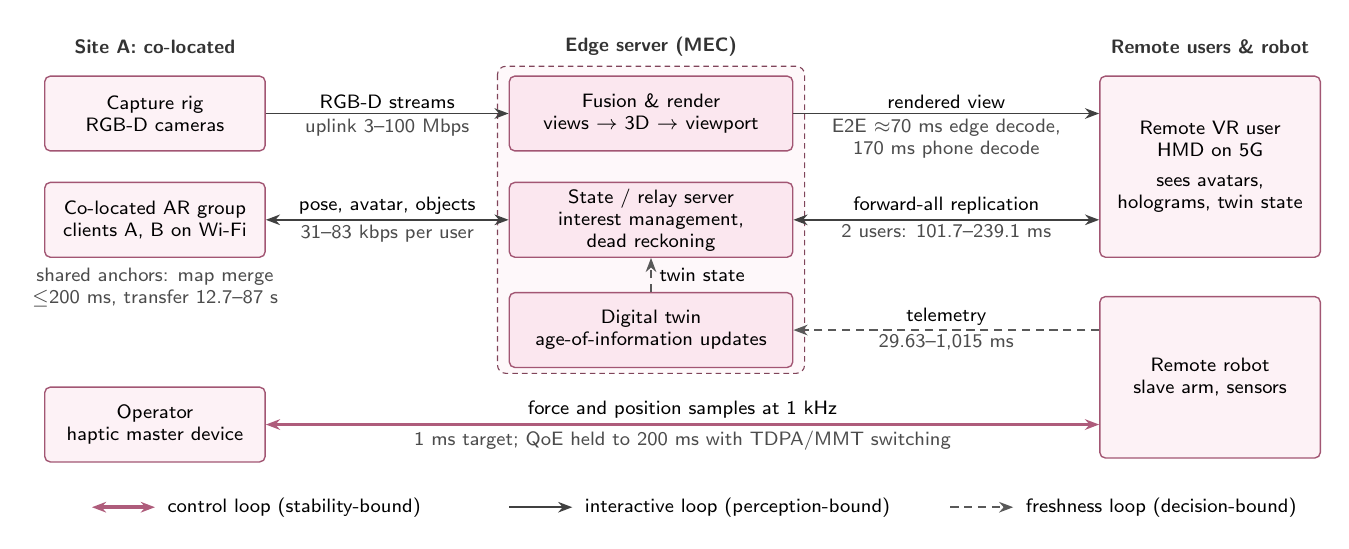
\begin{tikzpicture}[font=\sffamily\scriptsize, x=1cm, y=1cm,
  >={Stealth[length=1.8mm]},
  box/.style={draw=connect!70!black, fill=connect!10, rounded corners=2pt, align=center,
              line width=0.5pt, inner sep=2pt, text=black},
  ebox/.style={box, fill=connect!18, minimum width=3.6cm, text width=3.4cm, minimum height=0.95cm},
  lbox/.style={box, minimum width=2.8cm, text width=2.6cm, minimum height=0.95cm},
  ctrl/.style={<->, line width=1.3pt, draw=connect!75!black},
  inter/.style={line width=0.65pt, draw=black!75},
  fresh/.style={line width=0.65pt, draw=black!65, dash pattern=on 3pt off 2pt},
  lab/.style={font=\sffamily\scriptsize, align=center, text=black, inner sep=1.5pt},
  num/.style={lab, text=black!70},
  tier/.style={font=\sffamily\scriptsize\bfseries, text=black!80}]
% tier headers
\node[tier] at (1.4,0.85) {Site A: co-located};
\node[tier] at (7.7,0.85) {Edge server (MEC)};
\node[tier] at (14.8,0.85) {Remote users \& robot};
% edge tier background
\begin{scope}[on background layer]
  \fill[connect!5, rounded corners=3pt] (5.75,0.6) rectangle (9.65,-3.3);
  \draw[connect!55!black, line width=0.4pt, dash pattern=on 2pt off 1.5pt, rounded corners=3pt]
    (5.75,0.6) rectangle (9.65,-3.3);
\end{scope}
% left column
\node[lbox] (cap) at (1.4,0) {Capture rig\\RGB-D cameras};
\node[lbox] (grp) at (1.4,-1.35) {Co-located AR group\\clients A, B on Wi-Fi};
\node[num, below=2pt of grp] (anc) {shared anchors: map merge\\${\leq}$200~ms, transfer 12.7--87~s};
\node[lbox] (op) at (1.4,-3.95) {Operator\\haptic master device};
% edge column
\node[ebox] (fus) at (7.7,0) {Fusion \& render\\views $\rightarrow$ 3D $\rightarrow$ viewport};
\node[ebox] (st) at (7.7,-1.35) {State / relay server\\interest management,\\dead reckoning};
\node[ebox] (tw) at (7.7,-2.75) {Digital twin\\age-of-information updates};
% right column
\node[lbox, minimum height=2.3cm] (rem) at (14.8,-0.675) {Remote VR user\\HMD on 5G\\[3pt]sees avatars,\\holograms, twin state};
\node[lbox, minimum height=2.05cm] (rob) at (14.8,-3.35) {Remote robot\\slave arm, sensors};
% holoportation path (interactive)
\draw[inter, ->] (cap.east) -- node[lab, above] {RGB-D streams} node[num, below] {uplink 3--100~Mbps} (fus.west);
\draw[inter, ->] (fus.east) -- node[lab, above] {rendered view} node[num, below] {E2E $\approx$70~ms edge decode,\\170~ms phone decode} (fus.east -| rem.west);
% shared state (interactive)
\draw[inter, <->] (grp.east) -- node[lab, above] {pose, avatar, objects} node[num, below] {31--83~kbps per user} (st.west);
\draw[inter, <->] (st.east) -- node[lab, above] {forward-all replication} node[num, below] {2 users: 101.7--239.1~ms} (st.east -| rem.west);
% freshness loop
\draw[fresh, ->] (tw.east -| rob.west) -- node[lab, above] {telemetry} node[num, below] {29.63--1,015~ms} (tw.east);
\draw[fresh, ->] (tw.north) -- (st.south);
\node[lab, anchor=west] at ($(tw.north)!0.5!(st.south)+(0.05,0)$) {twin state};
% control loop
\draw[ctrl] (op.east) -- node[lab, above, pos=0.5] {force and position samples at 1~kHz}
  node[num, below, pos=0.5] {1~ms target; QoE held to 200~ms with TDPA/MMT switching} (op.east -| rob.west);
% legend
\begin{scope}[shift={(0.6,-5.0)}]
  \draw[ctrl] (0,0) -- (0.8,0); \node[lab, anchor=west] at (0.9,0) {control loop (stability-bound)};
  \draw[inter, ->] (5.3,0) -- (6.1,0); \node[lab, anchor=west] at (6.2,0) {interactive loop (perception-bound)};
  \draw[fresh, ->] (10.9,0) -- (11.7,0); \node[lab, anchor=west] at (11.8,0) {freshness loop (decision-bound)};
\end{scope}
\end{tikzpicture}
\caption{Architecture of a multi-party XR session: a co-located group and a remote user share state through an edge relay, a capture rig feeds edge fusion for holoportation, and an operator drives a remote robot whose digital twin updates every viewer. The loops differ in what bounds them (line style), so no single latency target serves the session. Numbers are measured values cited in the text: avatar rates and replication latency \cite{W4307020344}, holoportation rates and latency \cite{W4312662428,W4307263396}, anchors \cite{W4311118480,W4411499419}, twin updates \cite{W7213228059,W7168263637}, haptic rate and tolerance \cite{W2912555763,W2216406802,W4200154132}.}
\label{fig:connect-arch}
\end{figure}

\begin{table}[t]
\centering\small
\caption{The three loop types of a shared XR session. Measured tolerances come from the studies cited in the text; they show that each loop fails in a different way and needs its own network target.}
\label{tab:connect-loops}
\begin{tabularx}{\linewidth}{@{}>{\raggedright\arraybackslash}p{2.05cm}>{\raggedright\arraybackslash}X>{\raggedright\arraybackslash}p{2.0cm}>{\raggedright\arraybackslash}X>{\raggedright\arraybackslash}X@{}}
\toprule
Loop & What it carries & Bound & Delay measured or tolerated & Failure mode \\
\midrule
Control (haptic teleoperation) & Force and position samples at 1~kHz & Stability of the bilateral controller & 1~ms target; stable to 200~ms with TDPA/MMT switching \cite{W4200154132}, model-mediated to 1~s round trip \cite{W2811040154} & Oscillation or unsafe contact force \\
Interactive: shared state & Pose, avatar and object updates, tens of kbps per user & Perception of consistency and co-presence & 101.7--239.1~ms on deployed platforms \cite{W4307020344}; impairment noticed, task time unchanged \cite{W4392600587} & Divergent views, conflicting edits, unfair interaction \\
Interactive: remote people & Avatar parameters to volumetric video, 0.2--100~Mbps & Perception of the person & 70--170~ms end to end \cite{W4312662428}; avatar latency noticed at about 320~ms \cite{W4312899133} & Degraded, frozen or vanished person \\
Freshness (digital twin) & Telemetry and state of a physical asset & The viewer's decision & 29.63--1,015~ms, all reported adequate \cite{W7213228059,W7168263637} & Decisions taken on stale state \\
\bottomrule
\end{tabularx}
\end{table}

\subsection{Shared state: who holds the truth, and who sees what}

Every shared world must decide where the authoritative copy of its state lives and how much of it each client receives. Three families answer differently. \emph{Authoritative relays} order all updates at a server and forward them. Deployed social VR uses the simplest form: five commercial platforms forward every avatar update unprocessed, so throughput, latency and client load grow roughly linearly with users, and two-user end-to-end latency was 101.7--239.1~ms \cite{W4307020344}. A relay gives one ordering of events but puts itself in every path; routing through a cloud middleware raised round-trip time from 0.04~s to 0.6~s \cite{W4386499017}. \emph{Replicated, optimistic state} lets each client apply its own actions at once and reconcile later. Croquet-style virtual time \cite{W3174543121} and decoupled edge physics serving over 100 users \cite{W4404050807} belong here. They buy responsiveness and pay in conflicts: two users actuating one digital twin without a coordination policy conflicted in 33--56\% of time windows \cite{W7168268649}. \emph{Peer-to-peer and information-centric sharing} removes the relay. Named-data synchronisation \cite{W4404102246}, device-to-device exchange for web AR \cite{W3117560819} and co-located multicast, which rebuilt scenes several times faster than unicast TCP for groups of 7 and 16 \cite{W7147356863}, take this route. No study has compared the three families on the same workload.

Which inconsistencies users notice is assumed, not measured; consistency models appear only as concepts \cite{W3115046446,W2951580915}. Augmented Virtual Teleportation deliberately left its 1.2~s live video unsynchronised with avatar state to stay responsive \cite{W3005948101}. Yet synchronisation faults were the most common symptom in 2,649 bug reports from multi-user XR software \cite{W7166703064}.

Scaling fails at replication before it fails at link capacity. In a controlled study, update intervals grew from 18~ms with 2 clients to 158~ms with 125, and perceived fluidity collapsed beyond 25 avatars \cite{W2922194619}. Networked games use two remedies. Interest management sends each client only the state near or relevant to it. Dead reckoning sends a motion model and updates it only when the receiver's extrapolation error exceeds a bound. XR synchronisation has barely adopted either, and neither has been tested with XR users; lossy compression of joint rotations, a partial step, cut delay from over 300~ms to under 25~ms at 100~Hz \cite{W3008045703}. Large-scale claims rest on dummy clients \cite{W7130552889}.

Co-located AR adds a shared coordinate frame, which becomes the bottleneck. SPAR cut spatial inconsistency by up to 60\% by choosing what to communicate \cite{W3110126341}, and edge map merging finished within 200~ms \cite{W4311118480}, yet anchor transfers took 12.7--87.18~s \cite{W4411499419} and multi-user AR over public LTE had a 12.5~s median end-to-end latency \cite{W3047439371}.

Fairness between users is the most contested question. Edge schedulers minimise inter-player delay \cite{W4285149407,W3160366001}, and predictive buffering cut inter-client skew by 76\% for 100 clients in a controlled testbed \cite{W7168249167}. They assume that equal delay means equal experience. User evidence points elsewhere: dyads perceived network impairment but completed tasks no slower \cite{W4392600587}. The largest controlled study used 30 pairs \cite{W7163944086}, and a review of 56 studies found that almost all optimise latency for an individual, not a group \cite{W7154321690}. Group quality of experience (QoE), treated in \cref{sec:assure}, is unmeasured beyond pairs.

\subsection{People: a ladder of fidelity}

A remote person can be sent as a few joint angles or as a live volumetric capture; each rung up buys realism with bits, latency and capture hardware. \emph{Pose and parametric avatars} are cheapest: 24~B per update for a head pose and 216~B for a 17-joint skeleton \cite{W2922194619}, or 31--83~kbps per user on VRChat, Rec Room and Hubs \cite{W4307020344}. Expressiveness multiplies the rate; Horizon Worlds exceeded 4.5~Mbps downstream at 15 users \cite{W4307020344}. \emph{Semantic, model-driven avatars} send features that drive a pre-built model of the person. Mon3tr animated a Gaussian avatar with under 0.2~Mbps at about 80~ms \cite{W7123904049}, and MagicStream cut bandwidth up to 1,195-fold by sending keypoint and colour semantics \cite{W4404034698}. Apple's spatial personas use about 0.7~Mbps without rate adaptation \cite{W4403981191}. This family assumes an enrolled model and a stable feature stream; its robustness to loss is unsettled.

\emph{Volumetric telepresence} captures, uplinks, fuses and renders live geometry, and each stage has its cost. Raw point clouds of one person need about 300~Mbps; tiled user-adaptive streaming brought this to 14~Mbps \cite{W4304091566}. An operator trial streamed 5--100~Mbps, with end-to-end latency near 170~ms when phones decoded and 70~ms when the edge did \cite{W4312662428}; depth packed into H.264 needed 3--30~Mbps \cite{W4307263396}. Edge multipoint control units cut client load as parties grow \cite{W4387969165}. At the top, \emph{light-field booths} such as Project Starline \cite{W4200107448} need dedicated rigs; a full-duplex light-field link used 173~Mbps on a LAN \cite{W3176472668}.

Reusing the 2D real-time stack works: a WebRTC selective forwarding unit for point clouds adapted faster than TCP \cite{W7151958829}, and L4S converged on bandwidth 45\% faster than Google congestion control without frame loss \cite{W4408870658}. Two assumptions go unexamined. Calls are treated as downlink problems, yet only two studies measured the holographic uplink \cite{W4210904516,W4416047836}, and the operator trial attached its camera by Ethernet \cite{W4312662428}. Semantic schemes report savings in PSNR, never against geometry at equal bitrate with users. Whether 3D beats 2D is contested. Project Starline \cite{W4200107448} and stroke consultations with 30 outpatients \cite{W4400580381} favour 3D, while a floating-head prototype \cite{W7127277161} and a VR2Gather--Zoom comparison \cite{W4415708482} rated 3D below 2D video. All held the network fixed, although humanoid avatars lost more QoE under network distortion than cartoon ones \cite{W4415821547}.

\subsection{Touch: closing a control loop across the network}

Haptic teleoperation is the only loop here that closes a feedback system, so delay can destabilise it. The field set its requirement early at 1~ms end-to-end latency with 99.999\% reliability \cite{W2216406802}, and IEEE 1918.1 fixed a master--network--slave reference architecture \cite{W2911218692}. The requirement is costly at the radio: under finite-blocklength coding, transmit power becomes unbounded once the queueing-delay bound falls below the channel coherence time \cite{W2963776947}. Control theory offers three families that relax it. \emph{Wave variables} encode force and velocity so that the channel stays passive, but they handle only constant delay. \emph{Time-domain passivity} (TDPA) monitors the energy the network injects and dissipates it; with perceptual coding it stayed stable under time-varying delay of 100~$\pm$~30~ms while sending up to 80\% fewer packets. \emph{Model-mediated teleoperation} (MMT) renders force from a local model of the remote environment and sends only model updates; it cut data by about 90\% and stayed stable at round-trip delays up to 1~s \cite{W2811040154}. MMT assumes an environment that changes slowly enough to be modelled; TDPA suits fast-changing contact at low delay \cite{W2963793563}.

Perceptual coding is orthogonal to these families. Deadband coders send a sample only when the change would be felt, using Weber fractions of 7--15\% for force, and reduce packet rates by 80--90\% \cite{W2912555763}; codec details belong to \cref{sec:encode}. Prediction carries the same idea to the network: co-designing receiver-side prediction with radio resources saved up to 77.80\% bandwidth \cite{W4321488300}, and octree-based MMT raised force accuracy by 44\% with fewer than half the model updates \cite{W4401416073}. Both were evaluated open-loop on recorded or synthetic trajectories, not with a live network, a stable controller and users.

Measured tolerance is far looser and depends on the controller. Switching between TDPA and MMT held QoE at delays up to 200~ms \cite{W4200154132}, and users noticed short haptic delays but compensated \cite{W3162230828}. The 1~ms figure assumes a controller without delay compensation; it is not a measured limit of human touch. Transport results split by medium: a time-sensitive networking testbed kept high-priority flows at dedicated-wire quality under 200\% over-saturation \cite{W4387917733}, whereas Wi-Fi needs MAC changes that reached a 3.72~ms worst case for Wi-Fi~7 only in simulation \cite{W4205674533}. Haptic streams rarely travel with their video, and cross-modal work questions their usual priority: deliberate haptic loss with visual restoration raised opinion scores by more than 80\% at 30\% loss \cite{W4401507901}. Multi-user haptic studies stop at six pairs \cite{W4413393831}.

\subsection{Machines and places: keeping a twin fresh}

A digital twin reverses telepresence: the network must keep a replica of a physical asset fresh enough for the viewer's decision. The natural metric is age of information (AoI), the time since the newest received update was generated. Two families use it differently. \emph{Freshness optimisers} allocate radio and edge resources to minimise AoI or synchronisation time. They optimised AoI and reliability for short industrial packets \cite{W4366251214}, and optimal-transport association cut synchronisation time from 31.23--51.23~ms to 19.11--25.17~ms \cite{W4387870504}. They assume their workloads, such as 10~Mb per update \cite{W4387870504}, and rarely leave simulation; a task-oriented design on a real robot arm, which halved the required packet rate, is an exception \cite{W4390044355}. \emph{Measured pipelines} report what deployed stacks deliver. A robot vehicle mirrored on a headset updated in 29.63~ms over a local network \cite{W7213228059}, but middleware dominated elsewhere: 416~ms per transmission for a robot-arm VR twin \cite{W4417338851} and 1,015~ms end to end for a cobot through a commercial IoT platform \cite{W7168263637}. Each figure was called adequate; none was set against a task requirement.

Sending state rather than pixels is a consistent lever. Pose streaming kept remote work usable under added latency where video did not \cite{W4312316324}, a persistent twin with transient object updates allowed teleoperation at kilobits per second \cite{W4405784937}, and server push used three orders of magnitude less bandwidth than polling for a 5,005-building city twin \cite{W7172377742}. Once users act through the twin, the freshness loop becomes a shared-state problem, with the conflicts seen above \cite{W7168268649}. Freshness metrics have multiplied, yet none has been tested against what a viewer perceives or decides.

\begin{openproblems}
\item \textbf{What makes a group experience fair?} Skew schedulers assume equal delay means equal experience, but controlled studies stop at pairs \cite{W7163944086,W4392600587}. Groups of two to four under per-user impairments, scored on a shared task and perceived fairness, would give schedulers a validated target.
\item \textbf{Can interest management and dead reckoning scale social XR?} Platforms forward every update and scale linearly \cite{W4307020344}. Area-of-interest filtering with error-bounded extrapolation on an open platform, with a perceptual study of avatar error, would show how far replication cost can fall.
\item \textbf{How much delay does touch tolerate in XR tasks?} The 1~ms target persists while users tolerated 200~ms with adaptive control \cite{W4200154132}. Factorial delay, loss and jitter studies across TDPA, MMT and closed-loop predictors would yield tolerance curves for provisioning.
\item \textbf{How should haptic flows share a link with XR video?} Haptics and remote-rendered frames are scheduled apart. Joint scheduling on Wi-Fi or 5G, measuring haptic tail delay, motion-to-photon latency and inter-stream skew, would answer it.
\item \textbf{Which rung of the fidelity ladder serves a conversation?} Semantic avatars were never compared with geometry at equal bitrate, and 3D-versus-2D studies hold the network fixed. Two-way calls varying delay, loss and uplink rate against a matched 2D control are needed.
\item \textbf{How stale may a twin be?} AoI is optimised, yet no study links staleness to detection or control errors \cite{W4387870504,W7168263637}. Psychometric staleness curves for monitoring and actuation tasks would turn freshness budgets into requirements.
\end{openproblems}

\section{Assuring Experience and Trust: QoE, Security and Privacy}\label{sec:assure}

The previous sections optimise parts of the loop against targets. This section asks whether the result is
good enough for its users, and safe for them. Experience and trust share three properties. Both belong to
the whole loop: a frame arrives late because of the encoder, the scheduler, the transport pacing and the
reprojection together, and a pose leaks whether it travels to a renderer, a cache or a peer. Both are
judged at the human end, by what a user perceives and by what an adversary learns. And
both are usually inferred from proxies: network metrics stand in for experience, and attack accuracy on a
captured dataset for risk. The first half asks what users weigh and how experience and traffic
are modelled; the second asks what XR traffic reveals and what defences cost. \Cref{fig:assure-chain}
draws the measurement chain, the attack surfaces and the points where defences add delay.

\begin{figure}[t]
\centering
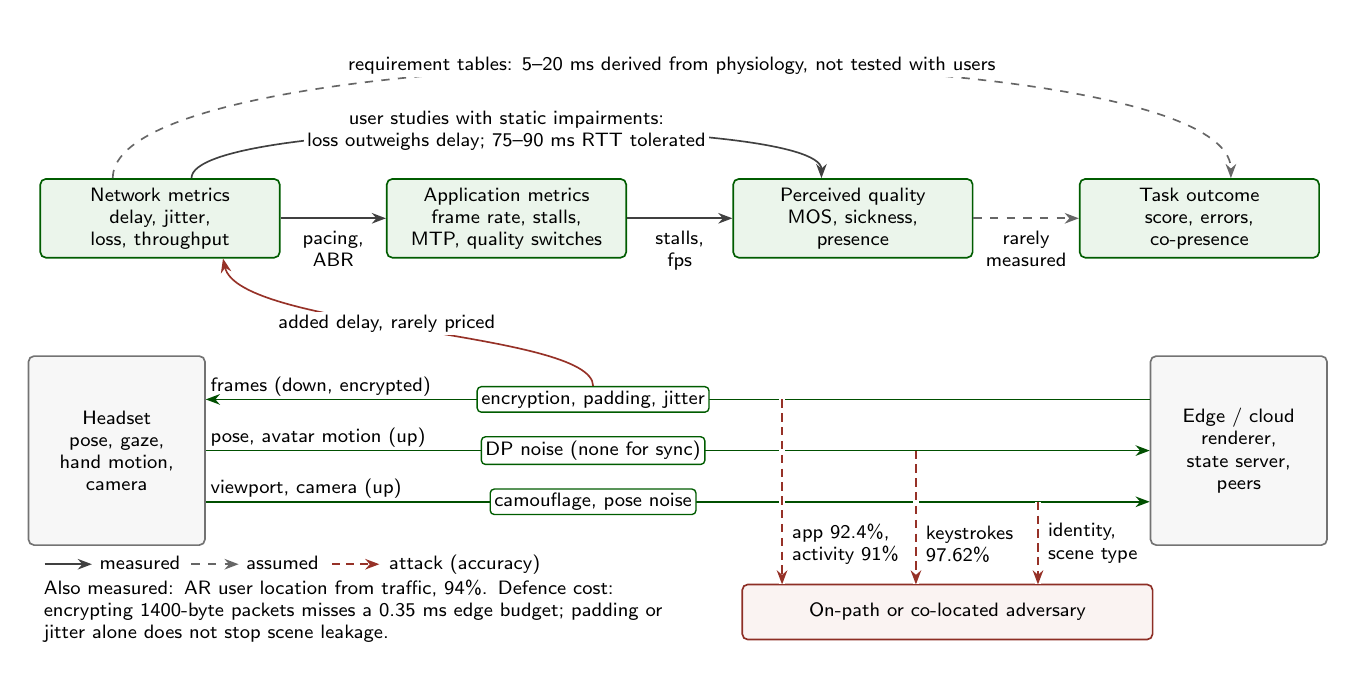
\begin{tikzpicture}[font=\sffamily\scriptsize,
  box/.style={draw=assure!70!black, fill=assure!8, rounded corners=2pt, align=center, text width=2.9cm,
    minimum height=10mm, inner sep=2pt, line width=0.6pt},
  sys/.style={draw=black!55, fill=black!3, rounded corners=2pt, align=center, text width=2.1cm,
    minimum height=24mm, inner sep=2pt, line width=0.6pt},
  adv/.style={draw=gapcolor!80!black, fill=gapcolor!6, rounded corners=2pt, align=center,
    minimum height=7mm, inner sep=3pt, line width=0.6pt},
  def/.style={draw=assure!70!black, fill=white, rounded corners=1.5pt, inner sep=1.5pt, line width=0.5pt},
  meas/.style={-{Stealth[length=1.8mm]}, line width=0.6pt, draw=black!75},
  assm/.style={-{Stealth[length=1.8mm]}, line width=0.6pt, draw=black!60, dashed},
  flow/.style={-{Stealth[length=1.8mm]}, line width=0.6pt, draw=assure!60!black},
  tap/.style={-{Stealth[length=1.8mm]}, line width=0.6pt, draw=gapcolor!85!black, densely dashed,
    preaction={draw=white, line width=2.2pt, -}},
  lab/.style={font=\sffamily\scriptsize, align=center, text=black}]
% --- measurement chain ---
\node[box] (n) at (1.6,0)  {Network metrics\\delay, jitter, loss, throughput};
\node[box] (a) at (6.0,0)  {Application metrics\\frame rate, stalls, MTP, quality switches};
\node[box] (p) at (10.4,0) {Perceived quality\\MOS, sickness,\\presence};
\node[box] (t) at (14.8,0) {Task outcome\\score, errors,\\co-presence};
\draw[meas] (n) -- node[lab, below=1pt] {pacing,\\ABR} (a);
\draw[meas] (a) -- node[lab, below=1pt] {stalls,\\fps} (p);
\draw[assm] (p) -- node[lab, below=1pt] {rarely\\measured} (t);
\draw[meas] ([xshift=4mm]n.north) .. controls +(0,0.8) and +(0,0.8) .. node[lab, fill=white, inner sep=1pt]
  {user studies with static impairments:\\loss outweighs delay; 75--90~ms RTT tolerated} ([xshift=-4mm]p.north);
\draw[assm] ([xshift=-6mm]n.north) .. controls +(0,1.9) and +(0,1.9) .. node[lab, fill=white, inner sep=1pt]
  {requirement tables: 5--20~ms derived from physiology, not tested with users} ([xshift=4mm]t.north);
% --- system and flows ---
\node[sys] (h) at (1.05,-2.95) {Headset\\pose, gaze,\\hand motion,\\camera};
\node[sys] (s) at (15.3,-2.95) {Edge / cloud\\renderer,\\state server,\\peers};
\draw[flow] (s.west |- 0,-2.3) -- (h.east |- 0,-2.3);
\draw[flow] (h.east |- 0,-2.95) -- (s.west |- 0,-2.95);
\draw[flow] (h.east |- 0,-3.6) -- (s.west |- 0,-3.6);
\node[lab, anchor=south west, inner sep=1pt] at (2.2,-2.3)  {frames (down, encrypted)};
\node[lab, anchor=south west, inner sep=1pt] at (2.2,-2.95) {pose, avatar motion (up)};
\node[lab, anchor=south west, inner sep=1pt] at (2.2,-3.6)  {viewport, camera (up)};
% defences on the flows
\node[def] (d1) at (7.1,-2.3)  {encryption, padding, jitter};
\node[def] (d2) at (7.1,-2.95) {DP noise (none for sync)};
\node[def] (d3) at (7.1,-3.6)  {camouflage, pose noise};
\draw[-{Stealth[length=1.8mm]}, line width=0.6pt, draw=gapcolor!85!black]
  (d1.north) .. controls +(0,0.7) and +(0.2,-0.9) .. node[lab, fill=white, inner sep=1pt, pos=0.55] {added delay, rarely priced} ([xshift=8mm]n.south);
% adversary and taps
\node[adv, text width=5.0cm] (x) at (11.6,-5.0) {On-path or co-located adversary};
\draw[tap] (9.5,-2.3)  -- (9.5,-4.65)  node[pos=0.78, right=0pt, lab, align=left] {app 92.4\%,\\activity 91\%};
\draw[tap] (11.2,-2.95) -- (11.2,-4.65) node[pos=0.70, right=0pt, lab, align=left] {keystrokes\\97.62\%};
\draw[tap] (12.75,-3.6)  -- (12.75,-4.65) node[pos=0.50, right=0pt, lab, align=left] {identity,\\scene type};
% legend and costs
\node[lab, align=left, anchor=north west, text width=8.3cm] at (0,-4.15) {%
  \tikz[baseline=-0.6ex]\draw[meas] (0,0)--(0.6,0); measured\enspace
  \tikz[baseline=-0.6ex]\draw[assm] (0,0)--(0.6,0); assumed\enspace
  \tikz[baseline=-0.6ex]\draw[tap] (0,0)--(0.6,0); attack (accuracy)\\[1pt]
  Also measured: AR user location from traffic, 94\%. Defence cost: \mbox{encrypting} 1400-byte packets misses
  a 0.35~ms edge budget; padding or jitter alone does not stop scene leakage.};
\end{tikzpicture}
\caption{Measurement chain and attack surfaces of a networked XR session. Solid arrows are links that user
or traffic studies have measured, dashed arrows links that are assumed; red taps show measured attack
accuracies, and defences sit on the flows where they add delay that has rarely been priced against the
frame deadline.}
\label{fig:assure-chain}
\end{figure}

\subsection{What users weigh}
Users of remote-rendered XR weigh loss and stalls above added delay of tens of milliseconds. On ALVR,
round-trip times (RTT) up to 90~ms were hardly noticed, while 8\% loss and a 35~Mbps cap degraded
experience \cite{W3095344018}. With CloudXR (N=30), QoE fell at RTT of 75~ms or more, at loss above 6\%,
or at 25~ms combined with 4\% loss \cite{W4402156718}. In social XR an RTT up to 77~ms had no significant
effect, while jitter did \cite{W4410087219}.

The headset separates two latencies. Rotation latency, the motion-to-photon (MTP) delay of turning the
head, is served locally by reprojection; network RTT reaches only interaction latency, the delay of
aiming, grabbing or seeing a peer react (\cref{sec:compute}). Isolated stalls of up to four frames went
unnoticed, and reprojection helped from eight frames (N=29) \cite{W4301184864}. This explains a contested
budget. Requirement papers derive 5--10~ms RTT and 20~ms interaction latency from physiology
\cite{W3035467795}, four to ten times below what users tolerated. No study has varied RTT and latency
compensation together, so the budget that edge placement should meet remains open.

The network moves perceived quality more than presence or sickness. Viewport-adaptive delay lowered
perceived quality but barely changed presence and left sickness almost untouched (20 observers)
\cite{W3037996690}. Fewer than 22\% of viewers reported sickness for AR point clouds, and two quality
levels were indistinguishable at 5~m on a HoloLens~2 (N=32) \cite{W4387831705}; content motion and
display, not the network, seem to drive sickness. Task performance is rarely measured beside
ratings. Group effects are tested almost only in pairs with
the impairment on one link \cite{W4415821547}; who is delayed in a larger group, and how the others judge
it, is unknown (\cref{sec:connect}).

These results share one study design: \emph{static impairments}. Every user study applies constant RTT,
independent loss or throttling; real 4G and 5G measurements enter only
afterwards, as inputs to models fitted under constant impairments \cite{W4405935991}. No study has
\emph{replayed measured network dynamics} to users. Wireless loss is bursty and correlated, so thresholds learned under independent loss may not transfer.

\subsection{How experience and traffic are modelled}
A QoE model maps what can be observed to what a user would report. Four families differ in what they
observe and what they were validated against (\cref{tab:assure-models}). \emph{Parametric standard models}
extend ITU-T P.1203 and P.1204.3 to tiled streaming \cite{W3200608537}, with P.919 as the test method for
short stimuli. \emph{Objective media metrics} are established for coding impairments: VMAF correlated best
on a public dataset \cite{W3115841380}, and colour PSNR reached $r=0.84$ for point clouds, depending on
content \cite{W4387831705}. Neither family sees interaction latency. \emph{Learned estimators} add it but
fit locally: a cloud VR gaming model reached a Pearson correlation of 0.93 \cite{W4400981668}. \emph{Network-side estimators} infer
quality from what an operator sees, such as encrypted 360-degree traffic from drive tests
\cite{W4384158049}, and are validated against formulas, not people. PERCEIVE predicted a parametric QoE
index within 4\%, but that index was never checked against ratings
\cite{W2809912305}.

\begin{table}[t]
\centering\small
\caption{Families of QoE models for networked XR. Each family is limited by what it observes and by the
ground truth it was validated against.}\label{tab:assure-models}
\setlength{\tabcolsep}{4pt}
\begin{tabularx}{\linewidth}{@{}>{\raggedright\arraybackslash}p{3.0cm}>{\raggedright\arraybackslash}X>{\raggedright\arraybackslash}X>{\raggedright\arraybackslash}X@{}}
\toprule
Family & Observes & Validated against & Limit\\
\midrule
Parametric standard (P.1203, P.1204.3 tiled) & Bitrate, resolution, stalls, quality switches & Ratings of short streaming stimuli & No interaction latency; 10~s stimuli\\
Objective media metrics (PSNR, VMAF, colour PSNR) & Decoded pixels or points against a reference & Ratings under coding impairments & Blind to timing; content dependent\\
Learned estimators & Network and application metrics, game state & Ratings on a few contents in one lab & Fitted and tested on the same small set\\
Network-side estimators & Encrypted traffic, radio and in-network counters & Parametric indices or activity labels & Never checked against users for interactive XR\\
Requirement tables & Human perception limits & Physiology, not networked user studies & 4--10$\times$ stricter than tolerated RTT\\
\bottomrule
\end{tabularx}
\end{table}

All four families lack \emph{temporal pooling}. P.919 uses 10~s stimuli, while presence needs
multi-minute tasks \cite{W4284879755}, and no model pools sub-second network events into the QoE of a
session.

\emph{Measurements of commercial platforms} show that the application stack, not the link, often sets what users see. WebRTC pacing in 5.56~ms batches set frame
delay at 6--21~ms over Wi-Fi~6 with an RTT of 1.5~ms \cite{W4391506055}. Under 27~Mbps throttling,
adaptive bitrate kept cloud VR frame loss at or below 5.12\% where a fixed 40~Mbps stream lost 32.51\%
\cite{W4210470894}: adaptation converts a throughput shortfall into image quality rather than lost frames.
Horizon Workrooms used 2--3~Mbps downlink and 0.6~Mbps uplink \cite{W4294643390}, two orders of magnitude
below the per-user rates in metaverse visions (\cref{sec:provision}). \emph{Statistical traffic models}
capture constant-bitrate video well, but they are open loop. The open RiftCat model matched mean but not
95th-percentile delay \cite{W3192844644}, and the 3GPP baseline underestimated effective VR bitrate by
25\% \cite{W4399340506}. None couples user motion with rate adaptation and congestion control, so
schedulers evaluated on them misjudge the tail.

\subsection{What XR traffic reveals}
XR transmits the body. Pose, gaze, viewport requests and camera frames are control signals and, at the
same time, behavioural and biometric data. Encryption hides content but not size, timing or
recipients.

\emph{Traffic metadata} reveals place and activity, an established result.
Traffic patterns of a mobile AR application located users with 94\% accuracy \cite{W2946752973}. On Meta
Quest Pro, off-the-shelf classifiers identified applications with 92.4\% accuracy and activities with
91\%, from under 10 minutes of traffic each \cite{W4406880464}. \emph{Motion as a
biometric} is the sharpest channel. Avatar motion received by an adversary's own client in multi-user VR
yielded 97.62\% of typed keystrokes across four applications \cite{W4398796475}, so state
synchronisation, which broadcasts head and hand poses to every peer, leaks by design
(\cref{sec:connect}). \emph{Viewport requests} identify users because prediction-driven tile requests
follow individual head motion (\cref{sec:anticipate}); the leakage persists under federated prediction
once prediction errors or QoE are uploaded \cite{W4223932369}. \emph{The camera uplink} of offloading AR
glasses reveals the type of physical scene through packet sizes and timing \cite{W7215028895}, so the
split chosen in \cref{sec:compute} is also a privacy decision.

\subsection{Defences and their price}
Every defence spends a resource the loop is short of: delay, bandwidth or prediction accuracy. The price
is rarely measured.

\emph{Encryption} is cheap for small packets and expensive at the tightest budgets: encrypting 1400-byte
packets did not fit a 0.35~ms edge budget, while 256-byte packets did \cite{W2923086750}.
\emph{Obfuscation} hides metadata at a cost in bandwidth or quality. Padding or jitter alone did not stop
scene leakage, and combined defences conflicted with QoS \cite{W7215028895}. Camouflaged tile requests
need more resources and degrade prediction \cite{W3207744807}. Noise remapping reduced the QoE loss of
privacy noise by 55--100\%, to 0--3\% at maximum privacy \cite{W4396941592}, but that loss is computed
from prediction accuracy; no user has been asked.

\emph{Authentication} schemes for
metaverse avatars are proven formally and costed in operation counts
\cite{W4295788720}; none is measured during an edge or platform hand-off, where re-authentication falls
on the interaction path (\cref{sec:provision}). \emph{Detection} rarely sees XR traffic: ``metaverse''
intrusion detectors report 96--99\% accuracy on IoT and enterprise datasets that contain no XR flows
\cite{W4388011607}. \emph{Blockchain} is contested: a 10-user pilot kept
88~FPS at 142 transactions per second \cite{W7161842864}, while most ledger frameworks report no latency
at all. The question is whether a ledger write sits on the interaction path.

The privacy--QoE trade-off is therefore modelled, not perceived. No testbed study reports a defence's
latency together with QoE or frame rate. A defence should be reported as a point on a privacy--QoE plane:
attacker accuracy against added 99th-percentile frame latency and bandwidth, on a real split-rendering
pipeline.

\begin{openproblems}
\item \textbf{Do network-side estimators predict what XR users report?} Estimators target parametric
  indices, and none addresses interactive remote rendering. A public benchmark pairing encrypted packet
  traces, client frame logs and per-minute ratings for cloud VR would let them be compared against people.
\item \textbf{Do thresholds from static impairments hold under real wireless dynamics?} Users have only
  seen constant RTT and independent loss. Replaying measured Wi-Fi and 5G traces, with reprojection on and
  off, would fix the latency budget for remote-rendered XR.
\item \textbf{How do sub-second events pool into session and group QoE?} No model links bursts of stalls
  to a multi-minute session, and groups beyond pairs are untested. Scripted burst schedules and asymmetric
  impairments in groups of four to six would answer both.
\item \textbf{Can a closed-loop traffic model reproduce the tail?} Open-loop models err at the 95th
  percentile. A generator coupling pose, rate adaptation and pacing, validated on several real headsets,
  would make scheduler studies credible.
\item \textbf{What does a defence cost against the frame deadline?} Measuring TLS, DTLS and QUIC with
  padding and jitter on split rendering, as attacker accuracy against 99th-percentile frame latency, would
  give providers a price; the same holds for re-authentication during hand-off.
\item \textbf{Can state synchronisation share avatars without sharing biometrics?} Broadcast poses reveal
  keystrokes. A protocol that perturbs or coarsens remote poses, tested for keystroke inference,
  co-presence and sickness, would close the channel.
\end{openproblems}

\section{Cross-Cutting Gaps}\label{sec:synthesis}

Read side by side, the open problems of the six functions repeat themselves in different vocabularies. Take
a viewport predictor never tested in a closed loop, an offloading controller that never left the
simulator, and an allocation scheme whose QoE objective was never shown to a user. They are three
instances of one shortfall. The atlas verified \nxrSynGapsTotal{} gaps across its \nxrDeepCells{} cells,
\nxrSynGapsHigh{} of them with high confidence. Nine themes account for \nxrSynCovered{} of them
(\nxrSynCoveredShare{}), including \nxrSynCoveredHigh{} of the high-confidence ones
(\cref{tab:themes}). A theme was kept only if it held gaps from at least six cells. We group the nine
themes into three families.

\begin{table}[t]
\centering\small
\caption{Nine cross-cutting themes. Gaps: verified cell gaps that instance the theme (high-confidence in
brackets). Cells: atlas cells in which the theme recurs. A gap can belong to more than one
theme.}\label{tab:themes}
\setlength{\tabcolsep}{4pt}
\begin{tabularx}{\linewidth}{@{}l>{\raggedright\arraybackslash}p{4.6cm}rr>{\raggedright\arraybackslash}X@{}}
\toprule
& Theme & Gaps & Cells & Indicative evidence\\
\midrule
\multicolumn{5}{@{}l}{\emph{Evidence foundations}}\\
T1 & No open traces, datasets or benchmarks & \nxrSynDataGapGaps{} (\nxrSynDataGapHigh{}) & \nxrSynDataGapCells{} & \nxrNDatasets{} dataset papers; \nxrSynReleaseShare{} of abstracts mention released code or data\\
T2 & Evaluation stops at the simulator & \nxrSynSimOnlyGaps{} (\nxrSynSimOnlyHigh{}) & \nxrSynSimOnlyCells{} & \nxrSynLearnedReal{} of \nxrSynLearnedN{} learning papers tested on a real network\\
T3 & Standards are not the evaluation substrate & \nxrSynStandardsGaps{} (\nxrSynStandardsHigh{}) & \nxrSynStandardsCells{} & \nxrSynThreeGPPXRN{} XR abstracts name 3GPP; none evaluated with users\\
\addlinespace
\multicolumn{5}{@{}l}{\emph{Objectives}}\\
T4 & Network metrics not linked to experience & \nxrSynNoQoEGaps{} (\nxrSynNoQoEHigh{}) & \nxrSynNoQoECells{} & \nxrSynQoEtermN{} abstracts invoke QoE; \nxrSynQoEtermUsers{} test it with users\\
T5 & Requirement figures inherited, not derived & \nxrSynRequirementsGaps{} (\nxrSynRequirementsHigh{}) & \nxrSynRequirementsCells{} & 1~ms target in \nxrSynOneMsN{} abstracts, \nxrSynOneMsUsersN{} tested with users\\
\addlinespace
\multicolumn{5}{@{}l}{\emph{Blind spots}}\\
T6 & Uplink and sending side neglected & \nxrSynUplinkGaps{} (\nxrSynUplinkHigh{}) & \nxrSynUplinkCells{} & ``uplink'' in \nxrSynUplinktermShare{} of abstracts, \nxrSynUplinktermSimAna{} of them simulated\\
T7 & Multi-user scale untested & \nxrSynScaleGaps{} (\nxrSynScaleHigh{}) & \nxrSynScaleCells{} & largest shared-world test: 225 clients \cite{W4400277138}\\
T8 & Security and privacy not costed & \nxrSynSecurityGaps{} (\nxrSynSecurityHigh{}) & \nxrSynSecurityCells{} & \nxrSynSecLatUsersN{} of \nxrSynSecLatN{} security--latency papers tested with users\\
T9 & Transport under real impairments & \nxrSynTransportGaps{} (\nxrSynTransportHigh{}) & \nxrSynTransportCells{} & \nxrSynXLFourSN{} corpus papers apply L4S\\
\bottomrule
\end{tabularx}
\end{table}

\subsection{Evidence foundations}
The first family concerns what claims are tested against. \emph{Data are missing} (T1). There are no
public traffic traces for AR offloading, avatar streams, twin-state updates, holographic calls or haptic
flows. No 360-degree dataset records head motion, network conditions and ratings in the same session,
and no latency benchmark couples motion, network delay and photodiode-measured MTP. Even simple
baselines are often missing: a persistence predictor reached a hit rate of 0.8355 against 0.8402 for a
sequence-to-sequence model on the same data \cite{W2963428739}. \emph{Evaluation stops at the simulator}
(T2). Whole technology lines, including reconfigurable surfaces carrying XR, terahertz XR links and
metaverse resource markets, have never met hardware. Where learned controllers were tested on unseen
users or content, they degraded \cite{W4403826584,W4400409717}. \emph{Standards are not used as the
substrate} (T3). 3GPP XR traffic models appear almost only in radio simulations. When one was checked
against measurement, it underestimated cloud-VR bitrate by 25\% \cite{W4399340506}. OMAF, MPEG Immersive
Video, IEEE~1918.1.1 and ITU-T P.1203/P.1204 are rarely the baseline configuration. The three gaps share
a cause. Collecting traces and building testbeds is costly, and venues that publish algorithms rarely
credit either.

\subsection{Objectives}
The second family concerns what is optimised. \emph{Network metrics are not linked to experience} (T4).
This is the largest theme. Most papers that optimise ``QoE'' optimise a formula whose weights were
chosen rather than fitted. Where users were asked, the answers diverged from the proxies. Packet loss
outweighed delay in VR cloud gaming \cite{W4404916373}. Users of collaborative VR could not tell forms
of latency apart \cite{W4392600587}. CloudVR users did not notice 20~ms of added latency
\cite{W2896076858}, while offloading papers optimise to budgets of 5--13~ms. \emph{Requirements are
inherited} (T5). Vision papers state 100--250~Mbps per metaverse user \cite{W4313291084,W4312940001},
while a measured commercial social-VR platform used 2--3~Mbps downstream \cite{W4294643390}. Holographic
requirements range from 5--100~Mbps for compressed calls \cite{W4312662428} to 6.63~TBps
\cite{W4300960574}. Haptic users tolerated up to 200~ms with adaptive control \cite{W4200154132}, against
the 1~ms figure that motivates much tactile-internet work. A requirement that names neither the
representation, the codec, the loop nor the percentile cannot be checked.

\subsection{Blind spots}
The third family concerns what is left out. XR sends a continuous upstream, yet the \emph{uplink} (T6)
is studied far less than the downlink, and the measured cases are pessimistic. On public LTE, multi-user
AR had a median end-to-end latency of 12.5~s, with the radio access network contributing 31.2\%
\cite{W3047439371}. With three headsets on Wi-Fi~6, uplink OFDMA delayed tracking data
\cite{W4396853623}. \emph{Scale} (T7) is untested. Measured social platforms scale linearly because they
forward all avatar data \cite{W4307020344}, and controlled QoE studies use pairs of users. \emph{Security
is not costed} (T8). Attacks are measured and effective: keystrokes were inferred from avatar motion with
97.62\% accuracy \cite{W4398796475}. Defences, however, are seldom priced in frame latency. \emph{Transport}
(T9) has not followed the move from buffered streaming to interactive delivery. Users rank loss above
delay \cite{W3095344018,W4404916373}, yet forward error correction and L4S are rare. An L4S pipeline for
volumetric conferencing converged 45\% faster than Google Congestion Control \cite{W4408870658}, but in a
controlled bottleneck.

\begin{figure}[t]
\centering
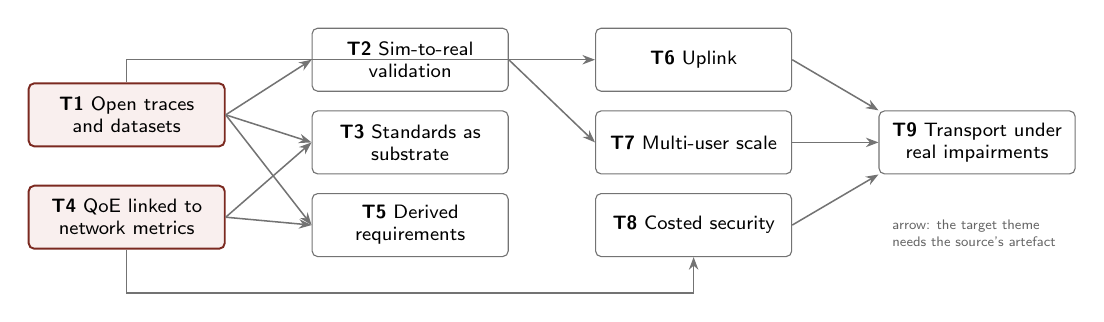
\begin{tikzpicture}[font=\sffamily\scriptsize,
  th/.style={draw=black!55,rounded corners=2pt,align=center,text width=2.35cm,minimum height=8mm,inner sep=2pt,fill=white},
  root/.style={th,fill=gapcolor!8,draw=gapcolor!70!black,line width=0.7pt},
  arr/.style={-{Stealth[length=1.6mm]},black!55,line width=0.55pt}]
  \node[root] (t1) at (0,0.55) {\textbf{T1} Open traces\\and datasets};
  \node[root] (t4) at (0,-0.75) {\textbf{T4} QoE linked to\\network metrics};
  \node[th] (t2) at (3.6,1.25) {\textbf{T2} Sim-to-real\\validation};
  \node[th] (t3) at (3.6,0.2) {\textbf{T3} Standards as\\substrate};
  \node[th] (t5) at (3.6,-0.85) {\textbf{T5} Derived\\requirements};
  \node[th] (t6) at (7.2,1.25) {\textbf{T6} Uplink};
  \node[th] (t7) at (7.2,0.2) {\textbf{T7} Multi-user scale};
  \node[th] (t8) at (7.2,-0.85) {\textbf{T8} Costed security};
  \node[th] (t9) at (10.8,0.2) {\textbf{T9} Transport under\\real impairments};
  \foreach \a/\b in {t1/t2,t1/t3,t1/t5,t4/t5,t4/t3}{\draw[arr] (\a.east) -- (\b.west);}
  \draw[arr] (t1.north) |- (t6.west);
  \draw[arr] (t2.east) -- (t7.west);
  \draw[arr] (t4.south) |- ++(0,-0.55) -| (t8.south);
  \draw[arr] (t6.east) -- (t9.north west);
  \draw[arr] (t7.east) -- (t9.west);
  \draw[arr] (t8.east) -- (t9.south west);
  \node[font=\sffamily\tiny,text=black!60,align=left,anchor=west] at (9.6,-0.95) {arrow: the target theme\\needs the source's artefact};
\end{tikzpicture}
\caption{Dependencies among the nine themes. Open traces (T1) and a validated mapping from network
metrics to experience (T4) are the roots. Without them, simulations cannot be validated, requirements
cannot be derived, and allocation, transport and security results cannot be compared in units that matter
to users.}\label{fig:themes}
\end{figure}

\subsection{How the themes depend on each other}
The themes are not independent (\cref{fig:themes}). Two are roots. Without open traces (T1),
simulations cannot be validated (T2), requirements cannot be derived (T5), standard traffic models cannot
be checked (T3), and uplink and multi-user workloads cannot even be described (T6, T7). Without a
validated mapping from network metrics to experience (T4), results on allocation, transport and security
(T8, T9) cannot be compared in units that matter to users. The two smaller clusters outside the themes
point the same way. Device-energy savings from offloading rest on models, and the few measurements
disagree: one standalone headset drained its battery 15\% faster when offloading wirelessly
\cite{W4362489903}, while an edge VR testbed found lower client power \cite{W4296339041}. Neural
scene representations have no tested rate adaptation, cache or split point. Both clusters need the same
two roots. This ordering shapes the agenda that follows.

\section{Research Agenda}\label{sec:agenda}

The gaps of \cref{sec:synthesis} suggest fourteen projects that a networking or multimedia laboratory
could start with existing hardware and open software. We order them by dependency (\cref{fig:roadmap}).
Projects that produce shared artefacts come first, because the others need them.

\begin{figure}[t]
\centering
\begin{adjustbox}{max width=\linewidth}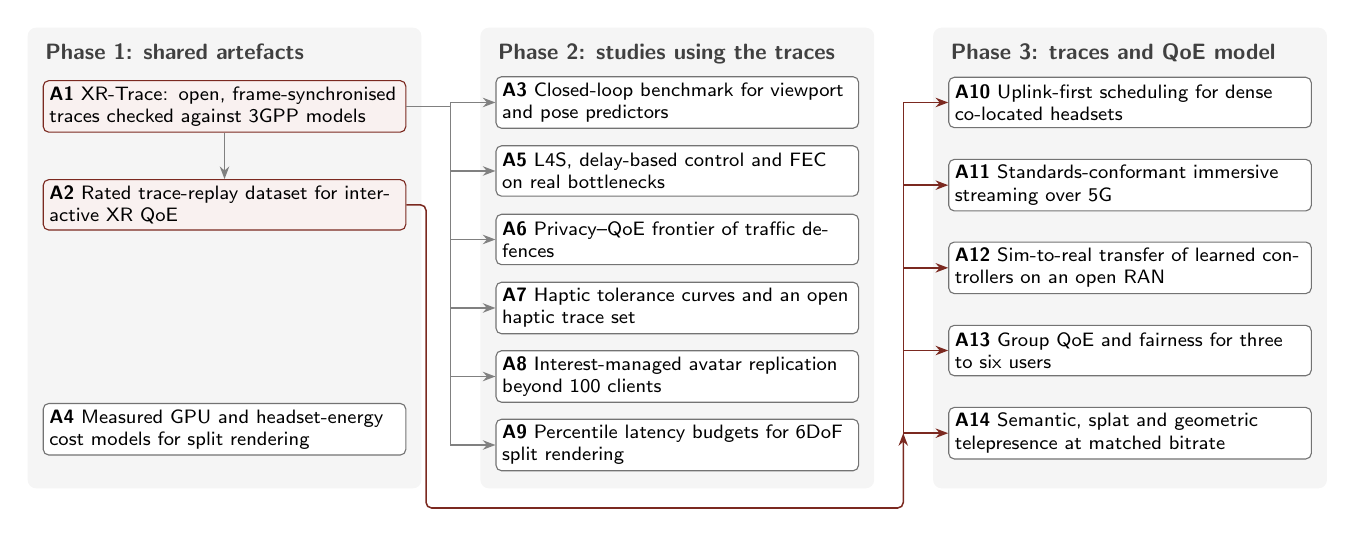
\begin{tikzpicture}[font=\sffamily\scriptsize,
  pj/.style={draw=black!55,rounded corners=2pt,fill=white,align=left,text width=4.45cm,inner sep=2.2pt,minimum height=6.4mm},
  ph/.style={font=\sffamily\footnotesize\bfseries,text=black!75,anchor=north west},
  arr/.style={-{Stealth[length=1.6mm]},black!50,line width=0.55pt}]
  \fill[black!4,rounded corners=3pt] (-0.15,0.5) rectangle (4.85,-5.35);
  \fill[black!4,rounded corners=3pt] (5.6,0.5) rectangle (10.6,-5.35);
  \fill[black!4,rounded corners=3pt] (11.35,0.5) rectangle (16.35,-5.35);
  \node[ph] at (-0.05,0.42) {Phase 1: shared artefacts};
  \node[ph] at (5.7,0.42) {Phase 2: studies using the traces};
  \node[ph] at (11.45,0.42) {Phase 3: traces and QoE model};
  \node[pj,fill=gapcolor!7,draw=gapcolor!70!black] (a1) at (2.35,-0.5) {\textbf{A1} XR-Trace: open, frame-synchronised traces checked against 3GPP models};
  \node[pj,fill=gapcolor!7,draw=gapcolor!70!black] (a2) at (2.35,-1.75) {\textbf{A2} Rated trace-replay dataset for interactive XR QoE};
  \node[pj] (a4) at (2.35,-4.6) {\textbf{A4} Measured GPU and headset-energy cost models for split rendering};
  \foreach \n/\y/\t in {a3/-0.45/{\textbf{A3} Closed-loop benchmark for viewport and pose predictors},
                        a5/-1.32/{\textbf{A5} L4S, delay-based control and FEC on real bottlenecks},
                        a6/-2.19/{\textbf{A6} Privacy--QoE frontier of traffic defences},
                        a7/-3.06/{\textbf{A7} Haptic tolerance curves and an open haptic trace set},
                        a8/-3.93/{\textbf{A8} Interest-managed avatar replication beyond 100 clients},
                        a9/-4.8/{\textbf{A9} Percentile latency budgets for 6DoF split rendering}}
    {\node[pj] (\n) at (8.1,\y) {\t};}
  \foreach \n/\y/\t in {a10/-0.45/{\textbf{A10} Uplink-first scheduling for dense co-located headsets},
                        a11/-1.5/{\textbf{A11} Standards-conformant immersive streaming over 5G},
                        a12/-2.55/{\textbf{A12} Sim-to-real transfer of learned controllers on an open RAN},
                        a13/-3.6/{\textbf{A13} Group QoE and fairness for three to six users},
                        a14/-4.65/{\textbf{A14} Semantic, splat and geometric telepresence at matched bitrate}}
    {\node[pj] (\n) at (13.85,\y) {\t};}
  \coordinate (b1) at (5.22,0);
  \draw[arr] (a1.east) -- (b1 |- a1.east) |- (a3.west);
  \foreach \t in {a5,a6,a7,a8,a9}{\draw[arr] (b1 |- a1.east) |- (\t.west);}
  \draw[arr] (a1.south) -- (a2.north);
  \coordinate (b2) at (10.97,0);
  \draw[arr,gapcolor!70!black,rounded corners=2pt] (a2.east) -- ++(0.25,0) -- ++(0,-3.85) -- (10.97,-5.6+0.0) -- (b2 |- a14.west);
  \foreach \t in {a10,a11,a12,a13,a14}{\draw[arr,gapcolor!70!black] (10.97,-5.1) |- (\t.west);}
\end{tikzpicture}\end{adjustbox}
\caption{Research agenda as a dependency roadmap. Phase-1 projects (red) build the artefacts that the
others consume. A1 supplies traces to every later project (grey arrows); A2, built on A1, adds the
validated QoE model that the Phase-3 projects optimise against (red arrows). A4 stands alone.}\label{fig:roadmap}
\end{figure}

\paragraph{Phase 1: build what others need.} \emph{XR-Trace} (A1) would instrument the main workloads on
5G standalone and Wi-Fi~6E/7, with one, four and eight users. These are split-rendered VR, AR camera
offloading, avatar and shared-state traffic, tiled 360-degree video and twin-state updates. Each trace
would record pose, encoder output, packets at both ends, application events and photodiode MTP on a
common clock. The project would then fit traffic models, compare them with the 3GPP XR models, and release
the traces with a replay harness for ns-3 and NetEm. It comes first because every
later project consumes it. The \emph{rated replay dataset} (A2) would have
participants perform interactive tasks while the network replays A1's traces. It would collect momentary
and session ratings, sickness scores, task performance and packet logs together, so that a QoE model can
be fitted and then used as the objective by other work. It would also measure the difference between
replayed dynamics and independent impairments of the same mean. \emph{Energy cost models} (A4) would
replace the assumed GPU and battery costs inside offloading optimisers with measured ones.

\paragraph{Phase 2 and 3: answer the open questions on shared ground.} With traces in hand, five
studies become cheap and comparable. They are a closed-loop predictor benchmark with persistence and
Kalman baselines (A3), transport on real bottlenecks (A5), a privacy--QoE frontier for padding and jitter
defences (A6), haptic tolerance curves (A7) and interest-managed replication beyond one hundred clients
(A8). A percentile latency budget for 6DoF split rendering (A9) completes the phase. With a validated QoE
model as well, the remaining projects can optimise against experience rather than a proxy. These are
uplink-first scheduling (A10), a standards-conformant 5G pipeline (A11), sim-to-real transfer of learned
controllers as xApps on an open RAN (A12), group QoE and fairness (A13), and a matched-bitrate comparison
of semantic, Gaussian-splat and geometric telepresence (A14).

\paragraph{The evaluation bar.} Each project should meet the standard that Transactions-level reviewers
apply, and that much current work does not yet meet. First, a \emph{baseline ladder}: a trivial baseline,
a classical method, the strongest recent method re-implemented under the same conditions, an ablation
and, where computable, an oracle. Second, \emph{realism with control}: real hardware for the claim and
trace replay for repeatability, with the gap between simulation and measurement reported. Third,
\emph{out-of-distribution tests} for anything learned, on held-out users, content and networks. Fourth,
\emph{sound statistics}: repeated runs with confidence intervals and, for user studies, a power analysis,
within-subjects designs and mixed-effects models. Fifth, \emph{reported cost and released artefacts}: run
time, energy and signalling overhead on the target device, with code, traces and analysis scripts
published.

\section{Conclusion}\label{sec:conclusion}

Networked XR has grown almost fourfold in eight years and has changed character on the way. It began as
a multimedia-systems field centred on 360-degree streaming. Its claims were tested with real players,
real traces and, often, real viewers. Today it is dominated by resource allocation, edge computing and 6G
architecture. It models XR traffic generically and tests most new claims in simulation. The empirical
core has not disappeared, but it has not grown with the rest. This core covers latency measurement,
multi-user and holographic systems, and QoE studies.

Organising the field by function makes the consequences visible. The functions that build systems,
compute and connect, rest on real testbeds in \fnComputeReal{} and \fnConnectReal{} of their papers.
Provisioning, now the largest and fastest-growing function, does so in \fnProvisionReal{}. Across all six
functions the same pattern recurs. Optimisers are well posed, but their inputs are assumed rather than
measured. The QoE they maximise was never shown to users. The requirements they meet were copied from
earlier surveys. The traffic they carry was synthesised.

The remedy is less a new algorithm than shared ground: open, frame-synchronised traces of real XR
workloads, and a QoE model fitted to people experiencing replayed network dynamics. With these two
artefacts, the questions that recur in every section become answerable on common terms: whether a learned
scheduler beats a heuristic on a real cell, how much latency a defence costs, and what a hologram really
needs. Without them, the field will keep growing faster than its evidence.


\bibliographystyle{ACM-Reference-Format}
\bibliography{data/references}
\end{document}
